%%This is a very basic article template.
%%There is just one section and two subsections.
\documentclass{scrreprt}

\usepackage{color}
\usepackage{hyperref}
\usepackage[automake]{glossaries}
\usepackage{tabularx}
\usepackage{rotating}
\usepackage{graphicx}
\usepackage{array}
\usepackage{lipsum}
\usepackage{placeins}
\usepackage{listings}
\usepackage[T1]{fontenc}
\usepackage{inconsolata}
\usepackage{float}
\usepackage{mfirstuc}

\usepackage[thinlines]{easytable}
\usepackage{enumitem}
\usepackage{longtable}
\usepackage{wrapfig}

\newcommand{\mn}{MicroNet} 
\newcommand{\ms}{microservice}
\newcommand{\mss}{microservices}
\newcommand{\msuc}{Microservice}
\newcommand{\mssuc}{Microservices}
\newcommand{\og}{online game}
\newcommand{\ogs}{online games}
\newcommand{\oguc}{Online game}
\newcommand{\ogsuc}{Online games}
\newcommand{\ogucuc}{Online Game}
\newcommand{\ogsucuc}{Online Games}

\newcommand{\code}[1]{\texttt{#1}}

\renewcommand*{\subsectionautorefname}{Subsection}
\renewcommand*{\subsubsectionautorefname}{Subsubsection}

%% \todo{} command.
%
% Outputs red TODOs in the document. Requires \usepackage{color}.
%
% Usage: \todo{Document the TODO command.}
%
% Comment out second line to disable.
\newcommand{\todo}[1]{}
\renewcommand{\todo}[1]{{\color{red} TODO: {#1}}}

\newcommand{\question}[1]{}
\renewcommand{\question}[1]{{\color{green} Question for Advisor: {#1}}}


\lstdefinelanguage{json}{
    basicstyle=\normalfont\ttfamily,
    numbers=left,
    numberstyle=\scriptsize,
    stepnumber=1,
    numbersep=8pt,
    showstringspaces=false,
    breaklines=true,
}

\definecolor{javared}{rgb}{0.6,0,0} % for strings
\definecolor{javagreen}{rgb}{0.25,0.5,0.35} % comments
\definecolor{javapurple}{rgb}{0.5,0,0.35} % keywords
\definecolor{javadocblue}{rgb}{0.25,0.35,0.75} % javadoc
 
\lstset{language=Java,
	basicstyle=\small\ttfamily,
	keywordstyle=\color{javapurple}\bfseries,
	stringstyle=\color{javared},
	commentstyle=\color{javagreen},
	morecomment=[s][\color{javadocblue}]{/**}{*/},
	numbers=left,
	numberstyle=\tiny\color{black},
	stepnumber=1,
	numbersep=8pt,
	tabsize=4,
	showspaces=false,
	showstringspaces=false
} 

\usepackage{authblk}

% Term definitions

\newacronym{mmo}{MMO}{Massive Multiplayer \og{}}

\newacronym{moba}{MOBA}{Multiplayer Online Battle Arena}

\newacronym{hsr}{HSR}{Hochschule f\"ur Technik Rapperswil}

\newacronym{soa}{SOA}{Service-Oriented Architecture}

\newglossaryentry{aaa}{name=AAA, description={
Triple A (AAA) is a designation of large games or large game development
companies. This term is commonly used in the game development industry.}}

\newglossaryentry{indy}{name={indy}, plural={indies},
description={Independent game development companies.}}

\newglossaryentry{sprite}{name={sprite},
description={2D representation of game objects. Sprites are 2D textures and
can optionally be animated.}}
 
\makeglossaries 

\begin{document}
 
\title{Microservices and Online Games}
\subtitle{Composition, Deployment and Development Concepts}
\author{Jonas Biedermann}
\affil{\vspace{1.5cm}\small{HSR - Hochschule f�r Technik Rapperswil}}
\affil{\small{Advisor: Olaf Zimmermann}}
\date{01.08.2017}
\maketitle

\section*{Abstract}
 
\setcounter{tocdepth}{1}
\tableofcontents 



\chapter{Introduction}

\section{Purpose of the Study}

The main purpose of this thesis is to incorporate the two research areas \mss{}
and \ogs{}. Both areas have individually been the topic of intense research
lately \todo{Citation needed} but no research exists on how to combine the two.

In regard to the \mss{} domain this thesis serves as a base for discussion about
\ms{} applications. Specifically the development and operation a set of \mss{} is
explained in detail. Of particular interest is the topic of how to facilitate
the composition of \mss{} and how to deploy a \ms{} application in a modern could
environment.

This thesis also provides a proof of concept that it is possible to
develop \ogs{} using \mss{}. For this purpose a vertical slice prototype is
developed to showcase the necessary fragments that make up a working \og{} in
the \ms{} world. Furthermore the prototype serves as a simple development
example of how to reproduce the development process of an \og{}. Is intended to
live on after this thesis ends and will continuously improved in the future.

As a secondary objective the usability of the recently very popular
\todo{Citation needed} Procedural Content Generation (PCG) is also discussed in
this thesis.

\section{Theoretical framework}

To curtail the infinite amount of research problems that the topics \ogs{} and
\mss{} offer a theoretical framework can be used. Within the framework the
abstract research problems are translated to research questions that cover the
area of interest sufficiently. According to the research questions hypotheses
can be formulated. The verification of these hypotheses is the final goal of
this thesis.

\subsection{Research Problems and Research Questions}

\subsubsection{Usability of a \ms{} for \ogs{}} 

\paragraph{Research Problem:} The usability of \ms{} suited to develop and
operate an \og{}.

\paragraph{Research Questions:}
\begin{itemize}
  \item Can an \og{} run in a pure \ms{} environment?
  \item Is a \ms{} influenced architecture suitable to design an \og{}?
  \item Is the added complexity during development tolerable?
  \item Is the overhead introduced by \mss{} negligible? 
\end{itemize}

\subsubsection{Deployment and Operation}

\paragraph{Research Problem:} The deployment and operation of a \ms{}
application in a cloud cluster-environment.

\paragraph{Research Questions:}
\begin{itemize}
  \item Which steps are necessary to operate an \og{} in a cluster-environment?
  \item How well do \ogs{} operate in a cluster-environment?
  \item How does a modern container engine assist in building and operating a
  \ms{} driven application?
  \item How can the deployment process be automated?
  \item Which tools exist that help the developer with deployment?
\end{itemize}

\subsubsection{\ms{} Composition}
\paragraph{Research Problem:} The composition of a set of \mss{} to form a coherent
distributed application.

\paragraph{Research Questions:}
\begin{itemize}
  \item What degree of composition is necessary for a \ms{} application to work?
  \item What is the minimal set of static and dynamic information that is needed
  for \ms{} composition?
  \item Which of the common paradigms orchestration and choreography is suited
  better for \ms{} composition?
  \item Which middle-ware is most useful in providing \ms{} composition?
\end{itemize}

\subsubsection{\ms{} Coupling}
\paragraph{Research Problem:} The degree to which \mss{} are semantically
dependent on each other. 

\paragraph{Research Questions:}
\begin{itemize}
  \item How can multiple game features be developed in parallel in different
  \mss{} while preserving the overall application behaviour?
  \item What problems are introduced by coupling game features loosely? 
  \item How does the consistency vs. performance trade-off impact \ogs{}?
  \item What protocols help to reduce service coupling?
  \item Can global static domain information help to reduce \ms{} coupling?
\end{itemize}

\subsubsection{\ms{} Development}
\paragraph{Research Problem:} The development process of a \ms{} application.

\paragraph{Research Questions:}

Development of a \ms{} application:
\begin{itemize}
  \item What separates \ms{} development from regular development?
  \item Which is the minimal number of steps ``from code to cloud''?
  \item Which tools help with \ms{} development?
  \item Which development tools make the development process significantly
  simpler?
\end{itemize}

\subsection{Hypotheses}

The essence of the research problems can be condensed to a set of hypotheses
which correspond with the different research areas. All hypotheses are
verified in the course of this thesis to prove that \mss{} are suited to
build an \og{}. 

\subsubsection{\ogs{} and \mss{} Hypothesis}
It is possible to build an \og{} as a pure \ms{} application by
respecting all seven \ms{} tenets.

\subsubsection{Required Features Hypothesis}
A minimal set of features is required to build a distributed \og{}: Networking,
persistence, serialization, session management and game engine integration.

\subsubsection{Stability and Performance Hypothesis} 
Microservices allow to separate the performance critical real-time game
simulation in regards to computing, bandwidth and latency requirements from the
non time-critical backend functionality of an online game. This allows arbitrary
scaling.

\subsubsection{Simple Development Hypothesis} 
Microservice can make the complicated process of developing online games simpler
by splitting up a complex game domain into small parts that can be developed
independently.

\subsubsection{Reproducibility Hypothesis} 
It is possible to completely prevent initial costs to kick of the development
process using only free/open-source technologies. This allows to reproduce the
development process anywhere at any time.

\section{Significance of the Study}

\mss{} are a very modern approach to realize a Service Oriented Architecture
(SOA). While SOA is not something new and has been in use for more then a decade
\todo{Citation needed} \mss{} are a cutting edge implementation approach to SOA
which has gained popularity only in the recent years. Therefore the theory and
references of how to actually develop and operate such a \ms{} environment are
rather sparse. This thesis servers as a complete reference for all relevant
aspects that have to be taken into account when an application (especially an
\og{}) is developed using \mss{}.

In regards to \ogs{} \mss{} have gained recent popularity. This is due to the
fact that large game development companies (>100 developers) prosecute \ogs{}
with million of player playing at the same time. For these games to scale the
traditional approach of running an \og{} as a monolithic application is not
sufficient. These large companies have large budgets at their disposal to
realize such an \og{}.

But this is not the case for smaller independent game development companies.
Independent companies are not constraint by founders and are therefor the main
driver for innovation in the game industry at the moment. But these  indy-teams don't
have the manpower to develop rich \ogs{} from scratch because the lack of
manpower and financial resources. Also AAA companies don't share their knowledge
about \og{} development to an extent that would allow indies to develop rich
\ogs{}.

Further \og{} development introduces the aspect of distribution within the game
application which is by definition a hard problem \todo{Citation needed}. There
is a lot of existing information on how to cope with asynchronism in game
development\todo{Cite: Gambetta}. However these references are mostly very low
level and leave a lot of responsibility to the developer. This added complexity
is whats holding back creative minds to develop rich \ogs{}. This thesis should
serve as a reference for these independent developers to gain a foothold in the
complex area of \og{} development.

\section{Definitions}

\section{Terminology Definitions}

\subsection{Simple Online Game}

A Online Game where where players are responsible to set up game servers. In
these environments the players make the game rules. Usually those are small scale
games which are played in a couple of session and the game state is saved
locally on the client. Examples are old LAN style games like for example Quake,
Age of Empires, or Diablo 2. If any online matchmaking exists for these games,
there is no centralized rule enforcement system in place.

\subsection{Rich Online Game}

These online games only require the player to download the game client or eaven
to just play it in the browers. That Game state of all players is stored on the
server infrastructure. A part from the game experience comes from this aspect of
an online managed game state. The rules must be enforced on the server
environment.

\section{Matchmaking}

Matchmaking is a process that helps players to find each other for an online
game. 


\section{Delimitations, Limitations, and Assumptions}

\chapter{Methods}

This thesis is the third and final part of a three semester project. The
substance of the past two theses was to build a foundation for the incorporation
of \mss{} and \ogs{}. 

The first project thesis consists of mostly literature about the topics \ogs{}
and \mss{}. The result is a comprehensive documentation of these two topics. The
essence of the document is the descriptions of a set of artifact that are
required to produce a fully functional \og{}.

During the second project thesis the theory established in thesis one was put
into practice. This was realized by implementing a prototype with the minimal
set of artifacts that are required to showcase the feasibility of \og{}
development with \mss{}. The results of the second project theses is a
feasibility study along with a fully functional prototype of an \og{} build
with \mss{}.

This third and final thesis is mainly about the elaboration of the previous tho
theses. This includes the examination of the open research problems listed in
\autoref{sub:problems} and the finalization of the prototype that was initially
developed during the second project thesis. This prototype serves as a reference
on how to develop and operate \ogs{} using a \mss{} environment.

\section{Subject Pool}
\label{sec:subject_pool}

The research problems that this thesis aims to solve are very variegated. To
gain an overview over all the activities that have to be conducted in the course
of this thesis the research problems can be collated to concrete subjects. These
subjects can then be examined individually.

\subsection{\ms{} Tenets in Relation to Online Games}

This is the major subject of this thesis and will therefore receive a lot of
attention. The research goal of this subject is to research every \ms{} tenet
according to its requirements in regards to \ogs{}. This is done in the form of
a requirements analysis of every tenet and a proposal on how to suffice them.
Examples for these solutions are implemented in the prototype and serve as a
demonstration. \todo{Ref to Result Section}

\subsection{Challenges Introduced by \mss{}}
\label{sub:ms_challenges}

It is challenging to suffice all \ms{} tenets for \og{} development. Most
noticeable the IDEAL tenet on specifically isolated state represents the biggest
challenge. This is because a game is always stateful. For example the location
of all chess pieces on a chess board is the state of the chess game. Since
\mss{} are always stateless the full game state must be sent with every game
message to provide true service confinement. In a simple game like chess this
might be possible but in a rich \og{} this is just no feasible. 

This challenge also exists in other computer science disciplines and is called
session management. In the case of \ogs{} sessions of players have to be
tracked but also the sessions of the game itself (e.g. one round of chess).

This challenge leads to another challenge namely game model access. Since the
game state is shared among multiple \mss{} a flexible approach is needed to
provide access to session data to the services.

The remaining challenges have already been discussed in the previous two project
theses.

\subsection{\ms{} Infrastructure}
\label{sub:infrastructure}

The \ms{} infrastructure subject is a collection of all topics that have to be
considered when operating a \ms{} environment. The content of this subject is
not restricted to the \ogs{} and can be applied to any domain.

\subsubsection{Requirements for \ms{} Composition}

The examination of the requirements for \ms{} composition can be grouped into
logical and physical composition (explained in \autoref{subsub:composition})
requirements.

The requirements for physical composition of \ms{} \og{} environments are very
similar to the requirements of classical business applications. The article of
O.Wolf provides a very good overview of the aspects of \ms{} composition and
discusses the paradigms orchestration and choreography in detail \cite{wolf_ms}.
Also C.Pahl and B.Lee provide a comprehensive paper that discusses requirements
to compose containerized applications in the cloud \cite{pahl2015containers}.

The requirements for logical composition are in essence very simple. Physical
composition offers a way for \mss{} to find each other. Logical composition is
on top of physical composition responsible that the services understand each
other.

\subsubsection{Deployment of a \ms{} Environment}

The deployment topic contains all aspects that have to be considered when a
production environment for a \ms{} application is realized. This includes the
continuous integration process that is responsible to build the application code
and deploy the executable files to the production environment.

Deployment also covers the aspect of choosing an appropriate cloud service
provider to that provides the physical infrastructure for the production
environment.

\subsubsection{Service Persistence}

The polyglot persistence approach proposed for \mss{} is only partially usable.
This is because a large portion of the state data (for example player data)
is essentially used by every service. With polyglot persistence only one
\ms{} would have direct access to this frequently requested data. This
inevitably leads to a bottle neck.

\paragraph{Durability}

In \ms{} environments databases are often deployed as \mss{} themselves.
Therefor it is in fact possible to loose the data stored in the containers. To
cope with this a durable solution is needed that adds a layer of redundancy to
guarantee that no data is lost. 

\subsubsection{Service Consistency}

One omnipresent problem with distribution is data consistency throughout the
application. For \ogs{} consistency is not as critical as like in for example
the medical industry but still undesirable. Also usually it is possible to spend
real money in an \og{} and therefore strong consistency is required for parts of
the application. 

\subsubsection{Service Monitoring}

In order to keep track on the health of a \ms{} application it is mandatory to
have live information on the status of the application. This includes a
visualization of the overall performance of the whole system and also for
individual services.

This topic also includes notification on events happening in the system like for
example notifications on system failure or regular operational reports. 

\subsection{Networking in \ogs{}}

Networking is obviously a critical part of \og{} development. it is important
that developers understand which implications the networked functionality has on
the game. Networking in video games is a well documented subject. An essential
reference for networking in \ogs{} is the blog of
G.Gambetta\cite{gambetta_fast_paced} about fast-paced multi-player. It is a
great reference to understand the low level aspects of networking in games.


\subsection{Development of a \ms{} Driven Online Game}

A number of tools in addition to the basic IDE can simplify the development
process of \ms{}. Many tools in this regard exist an can be of great value if
properly used. 

The following properties are desirable when selecting or developing tools:

\begin{itemize}
  \item Reduce the time needed to introduce new \mss{}
  \item Allow the developer focus on domain logic and not boilerplate code
  \item Increasing the automation level of continuous integration (deployment)
  \item Provide functionality to cope with \mss{} composition (both physical
  and logical composition)
  \item Visualization of operational statistics, communication flows and domain
  specific data like the game model.
\end{itemize}

\subsection{Procedural Content Generation in Online Games}

Procedural Content Generation (PCG) a strategy to produce game content
procedurally. PCG is an efficient way to reduce the effort needed by designers
to produce all the content needed for a game. Game content produced this way can
lack the desired quality and therefore manual intervention by game designers is
always required. PCG has become very popular in recent years
\cite{lee2014procedural} and is therefor a very interesting research topic in
regards to its usability for \og{} development.

PCG is usually realized using search-based methods. Especially evolutionary
algorithms perform very well. Some examples are: Fractal and noise algorithms,
grammars and L-systems, Planning algorithms, and many more. The book Procedural
Content Generation in Games \cite{shaker2014procedural} is a very comprehensive
summary on the topic which is currently widely researched in academia.


\section{Instrumentation}

As a first step to examine the subjects defined in \autoref{sec:subject_pool} a
clear definition of the technical foundation to reproduce the subjects during
the lab research (\autoref{sub:lab_reserach}) has to be made. For this purpose a
comparison of available technology is provided along with a proposal on how to
choose between similar available technologies.

\subsection{MicroNet: A Reference Implementation}

The prototype that has been already mentioned prior \todo{Exact reference}
several times is actually a collection of prototypes representing a reference
implementation on how to realize an \og{} using \ms{}.

The development title of this reference implementation is MicroNet.
MicroNet consists of the following components:

\begin{itemize}
  \item A core framework that provides run-time libraries required to operate a
  \ms{} \og{} application cluster.
  \item A small reference implementation on how to build an \og{} with MicroNet
  \item A service catalogue which contains reference implementation of
  functionality that is commonly uses in \ogs{}.
  \item A tool-set to simplify the development process of an \og{} 
\end{itemize}

\subsubsection{Common Functionality}

The polyglot programming tenet states that a \ms{} is free to choose its
implementation details. For the actual realization of a \ms{} application
this aspect introduces a number of challenges. 

It breaks the DRY (don't repeat yourself) principle if the same piece of
functionality is simply copied among multiple services. To cope with this a
solution is needed that on one hand does respect the DRY principle and on the
other hand provides a mechanism to share similar functionality among services.

One solution for this dilemma is to provide a reference solution that furnishes
a service with common functionality. This reference solution can be used to
build \mss{} which have no special technology requirement quickly.

In the prototype this aspect is tackled using a reference implementation
developed in Java. Java is in theory platform independent and therefore a good
choice to provide a general solution for \mss{} application design and
implementation. \mss{} with extended requirements are free not to rely on the
common solution and participate in the cluster autonomous.

\subsubsection{Application data}

As explained in \autoref{sub:games} an \og{} game operates on data. This data
must be suitable to be persisted and to be sent over a network (these aspects
have been discussed in project thesis 2 \todo{ref}). There is an literally
infinite number of ways on how to treat application data like for example Json,
XML, CVS, Strings, binary data, and HTML just to name a few.

Since \ogs{} are very time critical the fastest and therefore a binary data
format would introduce the least overhead. But since binary serialization
introduces a large amount of additional work during development it can be
considered an optimization\cite{gafferon2017games} and therefore a simpler data
format can be chosen for the prototype. Json is a good compromize in this regard
because it has an acceptable overhead, is human readable and also very popular.

\subsubsection{Networking}

An integral part of \ogs{} is networking. In regards of \mss{} the most common
approaches to networking are RESTful HTTP or Messaging. Messaging offers
several advantages over pure HTTP that are quite useful to make a \ms{}
application robust: Message queues are persistent and in case a service is
unavailable the messages are buffered and delivered as soon as the service
is available again. Furthermore it is possible to combine multiple message
brokers to a mesh to provide fail-over functionality. These aspects make a
message broker the optimal choice to facilitate networking for \ms{} \og{}
applications. Networking has been discussed in detail in project thesis one
\todo{Cite Thesis 1}.

\subsection{Development Environment}

The decision to propose Java as the main programming language for \mss{} allows
to derive a set of assumptions that simplify the development process of \ms{}
applications.

\subsubsection{Java as the Main Programming Language}

The latest Java Version 8 introduced functional programming into Java. With
functional programming it is possible to inject code into methods in a
convenient way. They are a perfect match to allow the developer to inject his
own code into a framework. MicroNet makes excessive use of this possibility.

Java enables the utilization of Apache Maven which is a very powerful software
project management and comprehension tool. It allows the describe and automate
the build process of a java applications. It also simplifies the process of
integrating third party java libraries into the application and the majority of
the java libraries are available as maven artifacts.

\subsubsection{Code Generation}

Java version 6 introduced annotation processing in the standard java build
process. This makes it very simple to provide framework functionality closely
related to the actual \og{}. Annotation processing coupled with code generation
are one major driver to facilitate the composition of \mss{}.

\subsubsection{The Eclipse IDE}

When it comes to Java development the Eclipse IDE is very popular. This is
backed by the fact that Eclipse has been around since \todo{Date} and has gone
though a long maturing process. Meanwhile Eclipse is a very robust development
environment not only for Java but also for many other programming languages. 

The way Eclipse is built makes it very easy to extend it. It is basically a set
of plug-ins that together form the IDE. The developer can write it's own
plug-ins to tailor the development process to his needs. 

MicroNet uses the Eclipse plug-in functionality to integrate \ms{} specific
development tools into Eclipse. With mininal effort it is also possible to
extract the MicroNet plug-ins to standalone applications. This however is out of
scope for this thesis.

\subsection{Container Engine}

Containers are a very powerful modern approach to run software. Instead of
installing a software directly on a host it is instead installed in a container.
The container can then run among other containers in a container engine as a
virtual machine. The container engine can be installed on any host that is
supported. This approach greatly increases the portability of software and
allows developers to build software once and run it anywhere as long as the
container engine is available.-

\subsubsection{Docker}

Docker is the most widely used container technology and a de-facto standard
\todo{Citation needed}. The docker ecosystem provides with Dockerhub a central
registry for available Docker containers. This centralized approach makes is
easy to install required dependencies on a system as long as docker is
installed.

\paragraph{Docker Compose}

Docker Compose is a way to describe a complex application consisting of multiple
Docker containers. With this approach it is possible to build or run a complete
\ms{} application with a single command. The structure of docker-compose is
also very well suited for automation. The compose script is in yaml format which
many libraries support.

Docker Compose is also the foundation to deploy a distributed application in
Docker Swarm explained in \autoref{sub:composition_engines}.

\paragraph{Docker for Windows}

As mentioned in \todo{Ref to Windows Requirement} the whole \og{} development
process must be realizable in Windows. Fortunately the Docker for Windows Client
is a very sophisticated tool that feels very close to the original Docker
version on Linux. One problem regarding Docker for Windows is that it does not
run on Windows versions which do not support HyperV. As a work-around developers
can use the Docker Toolbox. Docker Toolbox uses VirtualBox to provide the
same functionality as stand alone Docker but with the price of a little bit more
complexity during setup.

\subsection{Composition Engines}
\label{sub:composition_engines}

\subsection{Database Solution}
\subsection{Source and Artifact Control}
\subsection{Cloud Service Provider}










\subsection{Available Technology}

\subsubsection{Cloud Service Provider}

MicroNet is designed to run in the cloud. It is therefore mandatory to evaluate
the major cloud service infrastructure providers according to their usability
for online games.

One problem in regards to these service providers is payment. Although they
provide a free tier to test their infrastructure, a credit card has to be
pledged as security. In the case the limit is overdrawn a fee will be charged.
This risk cannot be taken in this thesis. 

\paragraph{Google Cloud Gaming Solutions}

Google offers a solution to deploy rich online games in the cloud. It basically
a setup for the existing google cloud infrastructure with additional
functionality to to provide build in matchmaking matchmaking. For this purpose
it provides an API that is available in a number of programming languages.

The MicroNet service that provides the matchmaking functionality has to be
altered if the Google solution for matchmaking wants to be used. 

To operate a game driven by MicroNet in the Google Cloud the Google App Engine
can be used to run the services of the MicroNet framework and the Google Compute
Engine can be used to run the game simulation servers. ActiveMQ that is used for
messaging can be used with Google Cloud by using Bitnami.

\paragraph{Amazon Game Lift}

Amazon GameLift is very similar to Google Gaming Solutions. It also provides a
matchmaking solution and the option to communicate with the game backend running
in the Amazon cloud. An advantage of the amazon solution is that it provides an
API for all the major game engines like Unity3D or Unreal Engine 4. Amazon also
provides its own game engine with the name Lumberyard.

\paragraph{A Dedicated Server}

The most general way to deploy the MicroNet framework is on a dedicated server
hardware. This could be either a cluster of bare metal servers with a sufficient
networking capabilities or a set of virtual servers running somewhere in the
cloud. Either way the result is a set of hosts running linux and have a public
ip address.

For this thesis a virtual server at the HSR will be the test setup. This
infrastructure is also available at the major cloud service providers.





\subsection{Game Engine}

\subsection{The Spacegame Prototype}



\section{Procedures}

The research methods used to examine the research problems explained in
\autoref{sub:problems} can be categorized into four areas: Literature
research, lab research, field research, and statistical analysis.

Each category provides a framework to enable research for one or more of the
more concrete research subject defined in \autoref{sec:subject_pool}. The table
below shows which research methods are used for each research subject.

\begin{center}
  \begin{tabular}{ l | c | c | c | c | }
  
  	&\begin{turn}{90}\textbf{Literature}\end{turn}
  	&\begin{turn}{90}\textbf{Lab Research}\end{turn}
  	&\begin{turn}{90}\textbf{Field Research}\end{turn}
  	&\begin{turn}{90}\textbf{Statistical}\end{turn}
  	\\\hline
    
    
    \textbf{Challenges Introduced by Microservices}&&x&x&\\\hline
    \textbf{Microservice Infrastructure}&x&x&&\\\hline
    \textbf{Networking in Online Games}&&&x&x\\\hline
    \textbf{Development of a Microservice Driven Online Game}&&x&x&x\\\hline
    \textbf{Procedural Content Generation in Online Games}&x&&&\\\hline
  \end{tabular}
\end{center}

The specific methods used in each category are derived from the design
science methodology principles\cite{wieringa2014design_science}.

\subsection{Literature Research}

Literature only plays a minor role in this thesis because the theoretical
foundation on \mss{} and \ogs{} has already been established in the last two
project theses. None the less literature is consulted in relevant areas to give
a theoretical backing to findings of this thesis.\\

Especially in the topic of \ms{} infrastructure a deep study of the
documentation of composition engines and cloud service providers was made
to highlight advantages and differences.\\

Since many sophisticated information about the \mss{} is shared via articles
and blog posts this type of references is considered valuable to back findings
with opinions of domain experts in the software industry.\\

in regards to \gls{pcg} the the book Procedural Content Generation In
Games\cite{shaker2014procedural} was studied in detail to identify \gls{pcg} methods
which are usable for \og{} development.

\subsection{Lab Research}
\label{sub:lab_reserach}

The majority of the research conducted during this thesis is lab research. This
is due to the very technical nature of the subject. 

The method used in lab research is the same for all research subjects namely
single-case experiments\cite{wieringa2014design_science}. Single-case
experiments examine one aspect of a problem domain under isolation.\\

Single-case experiments are conducted to examine all technical aspects of \mss{}
in regards to \ogs{} in a practical way. This includes the examination of the
\ms{} infrastructure requirements listed in \autoref{sub:infrastructure}, the
composition of \mss{}, the deployment of \mss{}, and the challenges introduced
by \mss{}.

All technical aspects can be examined on the basis of the instrumentation
artifact described in \autoref{sub:instrumentation}. The table below shows which
instrumentation artifact is used to examine each technical aspects.

\begin{center}
  \begin{tabular}{ l | l | l | l | l | l | }
    &\begin{turn}{90}\textbf{Composition}\end{turn}
    &\begin{turn}{90}\textbf{Deployment}\end{turn}
    &\begin{turn}{90}\textbf{Persistence}\end{turn}
    &\begin{turn}{90}\textbf{Consistency}\end{turn}
    &\begin{turn}{90}\textbf{Monitoring}\end{turn}
    \\\hline
    
    
    \textbf{MicroNet}&x&x&x&x&x\\\hline
    \textbf{Java as Programming Language}&x&&&&\\\hline
    \textbf{Application Data Format}&x&&x&x&\\\hline
    \textbf{Networking Technologies}&x&&&x&\\\hline
    \textbf{Container Engine}&x&x&&&\\\hline
    \textbf{Cloud Service Providers}&x&x&x&x&x\\\hline
    \textbf{Composition Engines}&x&x&&&x\\\hline
    \textbf{Database Solution}&&&x&x&\\\hline
    \textbf{Source and Artifact Control}&&x&&&\\\hline
    \textbf{Cloud Service Provider Gaming Solutions}&x&x&x&x&x\\\hline
    \textbf{Dedicated Server}&x&x&x&x&x\\\hline
    \textbf{Game Engine}&x&x&x&x&x\\\hline
    \textbf{Spacegame Prototype}&x&x&x&x&x\\\hline
  \end{tabular}
\end{center}

\subsection{Field Research}

To further back the findings gathered during the lab research field research is
conducted. But this is only possible to a limited extent because field research
is very preparation intensive. 

\subsubsection{Technical Action Research (TAR)}

Technical Action Research (TAR) allows to test a designed solution in a real
world context. This approach both gives the researcher a deep insight in the real
world problem domain. A secondary result of TAR is that the developed concepts
or designs can be used to help a stakeholder in real world projects.

TAR has been conducted in this thesis in the form of a series of play-test based
on the MicroNet and the Spacegame Prototype.

\subsubsection{Expert Opinion}

Expert opinion is used to validate the proposed development approach of
MicroNet. The experts solve a series of simple tasks with MicroNet and after
that share their impressions with a questionnaire. The chosen experts are master
students, game developers and software engineers.

\subsection{Statistical Analysis}

Since this thesis is mainly on exploratory basis the gathering of empirical data
has proven to be difficult. Especially the gathering of operational data from
field research is very cumbersome and also require a lot of effort to collect
the data and extract any meaningful information out of it. Because of this
reason the statistical analysis will be limited to the evaluation of the data
gathered during expert opinion validation.








\section{Statistical Analysis}

The results of the previous semesters are to this point only of hypothetical
nature. The main goal this semester is therefore to validate the findings up to
now.\\

Validation for the run-time aspect of the solution:

\begin{enumerate}
  \item To prove that the solution holds in regard to run-time is necessary to
  give proper validation feedback for the combination of Microservices and
  Online Games. It must be shown the running framework is able to scale at
  run-time. In a first instance this is done by performing lab-research in the
  form of small scale play test with some elected test players.
  \item One more sophisticated approach is to perform TAR on the run-time
  validation. This would mean to test the MicroNet with the alpha version of the
  Spacegame prototype in a long running tests that is available for the public. 
\end{enumerate}

Validation of the development-time aspect of the solution:

\begin{enumerate}
  \item It must be proven that the proposed development solution is actually
  usable and as simple as proposed.
\end{enumerate}

This validation research is made according to design science methods and
teminology.



















\chapter{Results}

This thesis aims to deliver results which are useful in practice and not only
of theoretical value. To make the results practically relevant a lot of effort
has been invested in the MicroNet prototype which serves as a reference
implementation for the concepts developed in this thesis.

\section{Order of Presentation}

The results are all presented together with a specific part of the MicroNet
prototype. The different areas in which results are worked out are all related
to the research problems explained in \autoref{sub:problems}. These areas are:

\begin{itemize}
  \item Proposition for an  open source technology stack to fully build and
  deploy a \og{} driven by \mss{}
  \item MicroNet as a reference implementation of a \ms{} \og{} development and
  operation framework using the proposed technology stack
  \item Validation of the practicality of the framework using data gathered with
  an expert survey 
\end{itemize}

\section{Technology Stack}

The feature hypothesis (\autoref{sub:hypothesis}) states that networking,
persistence, serialization, session management and game engine integration are
necessary to build a fully functional \og{}. These essential features are
mandatory to drive an \og{}.

In addition to these core technologies, supplementary technologies are needed to
help fulfill the deployment and the simple development hypothesis
(\autoref{sub:hypothesis}). These technologies are: container engine,
composition engine, continuous integration solution, source control system, and
\glsreset{ide}\gls{ide}.

The rest of this section describes each technology and states advantages and
disadvantages along with the arguments which are decisive for the composition
of the technology stack.

\subsection{Core Technologies}

The core technologies have mostly been defined and tested in the prior two
project theses. This section only gives a short summary on the chosen
technologies.

\subsubsection{Networking}

\begin{wrapfigure}{r}{4cm}
	\vspace*{-0.2cm}
    
\includegraphics[width=4cm]{images/dependencies/activemq}
\end{wrapfigure}

\textbf{ActiveMQ} is a popular message broker. A message broker buffers
messages and delivers them as soon as a receiver is available. This allows for a
robust and persistent messaging. Message brokers have been evaluated during
project thesis one. ActiveMQ is the networking foundation of MicroNet and
has proven to be very stable. ActiveMQ is supplied with a Java JMS library which
provides a way to easily integrate ActiveMQ into Java applications.

ActiveMQ is available on Docker Hub as a Docker image and can therefore easily
be integrated into a \ms{} application using a composition engine.


\subsubsection{Persistence and Session Management}

\begin{wrapfigure}{r}{4cm}
 	\hspace*{0.4cm}
    
\includegraphics[width=4cm]{images/dependencies/PostgreSQL}
\end{wrapfigure}

\textbf{PostgreSQL} is a very mature open source relational database. It is
available on all major platforms, which allows for comfortable testing and
deployment. Since version 9.2 PostgreSQL supports the \gls{json} data-type,
which makes it trivial to control the data flow from the network to the database.

PostgreSQL is also available on Docker hub and can therefore be quickly
integrated. For production purposes a native installation of PostgreSQL is
suggested to provide the needed stability as explained in
\autoref{sub:database_solutions}.\\ 


\begin{wrapfigure}{r}{4cm}
    
\includegraphics[width=4cm]{images/dependencies/couchbase}
\end{wrapfigure}

\noindent \textbf{Couchbase} is a NoSQL database realized as a \gls{json}
document store. The \gls{json} affinity of Couchbase cooperates very well with
the technology stack. Couchbase has its own query language called N1QL which
allows aggregated queries between multiple documents. Also access on
sub-document level is possible to allow fine grained data access.

Couchbase can run in a cluster and maintains a quorum on each document to
provide eventual consistency on document write operations. The cluster
functionality can be used to scale the database system. Couchbase also provides
timeouts of documents which can be used to imitate \textit{session store}
behaviour to facilitate session management. This neglects the need for a
distributed caching system like Redis.

Even if Couchbase exists as a Docker image it is advised for production to
install a native version of Coutchbase for the reasons explained in
\autoref{sub:database_solutions}. For testing the containerized version can be
very helpful due to the quick setup. This is further supported by the fact that
Couchbase is schema-less which further simplifies the installation process. 
    
\newpage
\subsubsection{Serialization}

\begin{wrapfigure}{r}{4cm}
    
\includegraphics[width=4cm]{images/dependencies/google-gson}
\end{wrapfigure}

\textbf{Gson} from Google offers a very convenient out-of-the-box approach to
serialize Java objects to \gls{json} strings and vice versa. It is an additional
advantage of Gson to supports generic collections like hash-maps.

The main advantage of Gson is its simplicity. The simplicity happens at the
expense of of performance especially for the de-serialization of \gls{json}
Strings. Because of this reason simple Gson serialization is only useful in
areas where a performance hit does not influence the application behaviour.

\subsubsection{Game Engine Integration}

\begin{wrapfigure}{r}{4cm}
    
\includegraphics[width=4cm]{images/dependencies/Unity3D}
\end{wrapfigure}
    
\textbf{Unity3D} is very popular among independent developers because it has no
initial financial barrier. Unity3D is very well documented and has a very
healthy community to provide support for development problems.

Unity3D provides a rich editor that may be used to prototype games quickly. It
also offers a rich C\# \gls{api} which is used to write any imaginable game
simulation logic.

For this thesis it is of particular interest to see how well the combination of
C\# game logic and Java back-end logic works in regard to the \ms{} tenet of
polyglot programming.
    
\subsection{Supplementary Technologies}

The supplementary technologies have been under intense evaluation during the
process of this thesis. The result of this evaluation is a set of augmenting
technologies which work well together, are easy to learn, and are open source or
have a community edition (free of charge and maintained by the community).

\subsubsection{Container Engine}

\begin{wrapfigure}{r}{4cm}
	\vspace*{-0.5cm} \hspace*{0.2cm}
    
\includegraphics[width=3cm]{images/dependencies/docker}
\end{wrapfigure}

\textbf{Docker} has already been mentioned several times in this document.
The essence about Docker is that it is an enabler technology. This is because
all other composition and container technologies support Docker in some way.
This aspect makes Docker Engine a reliable intermediate layer between the actual
hardware and the application running on it.

\newpage
\subsubsection{Composition Engine}

\begin{wrapfigure}{r}{4cm}
	\vspace*{-0.5cm} \hspace*{0.8cm}
    
\includegraphics[width=2.4cm]{images/dependencies/docker-compose}
\end{wrapfigure}

\textbf{Docker-compose} is basically only a CLI application which translates a
docker-compose file into a set of docker commands which are sequentially
executed. The result is a containerized application running on a single
host. Docker-compose is very helpful to quickly deploy a \ms{} application
stack locally. The docker-compose format also provides the basis to deploy a
composed application in the cloud using docker-swarm.\\

\begin{wrapfigure}{r}{4cm}
	\hspace*{0.4cm}
    
\includegraphics[width=3.3cm]{images/dependencies/docker-swarm}
\end{wrapfigure}

\noindent\textbf{Docker-swarm} is used to run containerized applications on a
cluster of Docker machines. A Docker machine is simply a host running a Docker
engine. Docker swarm allows to deploy each services of an application
individually using the docker stack CLI and also offers the possibility to
deploy a complete application stack defined through a docker-compose file.
Docker swarm offers multiple scheduling strategies which distribute the
containers among the available docker machines.

The major advantage of Docker swarm is its simplicity. Only a few commands are
needed to control the cluster so docker-swarm is therefore easy to understand.
Since it is the native Docker composition technology it is also a natural match
for containerized Docker applications.

One noticeable disadvantage is the lack of several convenience features like a
build-in dashboard or auto-scaling support. This is not a big concern since many
third party dashboard tools like Grafana are available and auto-scaling can be
added with a little bit of an implementation effort.

\subsubsection{Continuous Integration}

Continuous integration is generally a part of every software project and \ogs{}
are no exception. In this thesis the continuous integration process is examined
up to the point where all individual steps of the process are defined. From here
a central build system like Jenkins can take over and unify the whole build
process, but this aspect is not covered in this thesis.\\

\begin{wrapfigure}{r}{4cm}
    
\includegraphics[width=4cm]{images/dependencies/maven}
\end{wrapfigure}

\noindent\textbf{Maven} is a build system and provides a convenient way to
define the build process of Java applications. For the game back-end services
which are mainly written in Java this is a perfect match to define the build
process.

Maven also works very well in cooperation with Docker. A dedicated Maven Docker
image can be used to easily integrate the Java build process into the Docker
build process by executing the Maven build inside the target container. This approach
removes the need of any local Java or Maven installation. 

The drawback of the complete in-container Maven build is its performance.
Maven downloads ``the whole Internet'' into every container to build the
application. This is not useful during development where short build times are
mandatory. In order to cope with this problem the Maven build can be conducted
on the host system and only the binaries (executable Jars in case of Java
services) are sent to the Docker daemon for the container build process. This
makes the combined build process much faster and has no real disadvantage
because the process can be exactly reproduced on the build system and therefore
also speeds up automated builds.

Maven is also very useful to preserve a consistent versioning of \mss{}. The
game application stack can be described using a master .pom file containing
the required versions of all services. The master .pom file can be updated to
introduce a new version of any service. The continuous integration process can
be triggered at this point to perform a rolling update of the currently
deployed application stack.\\
	


\subsubsection{Source Control System}

A source control system is mandatory in every software project to keep track of
artifacts and versions. Source control is important to safely store the source
code of an application but also to provide source level access to many open
source projects like MicroNet.\\

\begin{wrapfigure}{r}{4cm}
    
\includegraphics[width=4cm]{images/dependencies/github}
\end{wrapfigure}

\textbf{Git} is the \textit{Source Control System} that builds the foundation
for the version control. Git works perfectly to share Maven projects which in
turn is used to reproduce the build process locally and also on a build server.

Github is used to provide any needed dependency used for the build process.
MicroNet is also published via Github.

\subsubsection{Interactive Development Environment (IDE)}

\gls{ide} is a wide term for a tool that simplifies the development process of a
software program. Usually it provides comprehensive tools that assist in writing
the source code of an application.\\

\begin{wrapfigure}{r}{4cm}
    
\includegraphics[width=4cm]{images/dependencies/eclipse}
\end{wrapfigure}

\noindent\textbf{Eclipse provides} a very solid \gls{ide} to develop Java
projects. The plug-in development environment of Eclipse can be used to
customize the \gls{ide} to an arbitrary extent. This aspect is especially useful
because almost no specific \ms{} development tools are available on the market.
Also Eclipse provides a number of very useful plug-ins for Java development.

The \textit{Docker Tools} for Eclipse consist of a visual explorer for Docker
images and containers. It allows to quickly start, stop, build and remove containers
without having to bother with console commands.

\textit{Launch Groups} is a plug-in contributed by Eclipse CDT (C++ development
plug-in for Eclipse). It is very useful to directly run or debug multiple
applications at once. This allows to quickly bring up or terminate the whole
application stack for testing purposes. Although CDT is required for Launch
Groups it does not interfere with Java development.
































\section{MicroNet}

MicroNet is a framework to develop and operate \ms{} applications. It is
designed to be especially support rich \ogs{} but is not restricted to this
domain. MicroNet also provides all needed tools and examples to showcase how to
develop and operate an \og{}.

\subsection{Characteristics of MicroNet}

To reduce the complexity of an \og{} development a \ms{} approach can be used by
splitting the domain of a game game into small shards that can be developed
independently. These shards are defined using a \glsreset{ddd} \gls{ddd}
approach. This is the general concept behind MicroNet.\\

In addition to the general concept MicroNet is designed according to four
guidelines to provide a lean and agile \og{} development process:
\begin{itemize}
  \item MicroNet does not reinvent the wheel for online game development but
  instead makes use existing technologies, specifically popular game engines
  \item MicroNet tries to make the developer aware of the problems that are
  encountered during the development process as early as possible
  
  \item Using MicroNet aims to help the developer to learn the process of \og{}
  development and solve related problems
  \item MicroNet supports the developers in realizing the especially
  difficult aspects of communication and consistency in a \ms{} application
\end{itemize}
\subsection{Realizing \ogs{} with MicroNet}

\begin{figure}
	\centering
	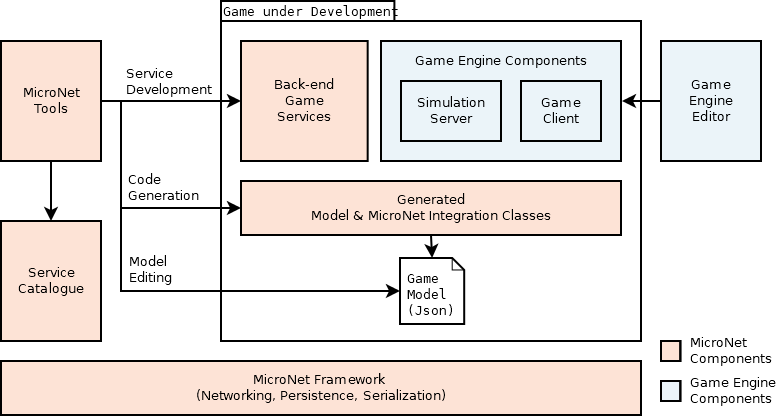
\includegraphics[width=\textwidth]{images/architecture/GameWithMicroNet}
	\caption{The MicroNet setup for \og{} development.}
	\label{fig:game_with_micronet}
\end{figure}

\autoref{fig:game_with_micronet} shows how the MicroNet development setup for an
\og{} looks like. The game model is represented by Json files and is used to generate
the classes needed to participate in a MicroNet application. This allows the
integration of the back-end game services but also of the game simulation
server and the client into the application. Back-end can also bypass the
generated integration layer and directly use the framework functionality. 

The game engine components are developed using the game engines regular
development workflow. The integration of MicroNet can be achieved by either
mirroring the framework integration generation in the language of the game
engine or manually program the integration classes.

A disadvantage of this setup is that the framework integration layer has to be
realized for all used technologies. This introduces quite an overhead but is
compensated by the improved work-flow which is possible once the integration is
done. It has to be mentioned that the implementation effort to realize the code
generation part which generates the framework integration classes is rather
small. The model definition and editing take care of most work in this regard.
The code generation layer is only responsible to generate simple classes out of
the well defined Json model files which is a very doable task and well
documented through the MicroNet code generation plug-in which serves as a
reference implementation. Also the developer has always the choice to integrate a foreign
technology into MicroNet by using only ActiveMQ as the message broker bypassing
the integration layer. ActiveMQ is very portable since it offers many clients on
many platforms.

With the integration layer out of the way the developer is free to use the
MicroNet tools to speed up and clarify the development process. This includes
the possibility to integrate reference services from the service catalogue into
the application. It also includes the possibility to use MicroNet core
features like networking, persistence, and serialization.

\subsection{Architecture Overview}

The MicroNet framework is a collection of components. Each component is
confined in itself which allows simple replacement of components. The components
are organized in three layers: The framework layer, the service catalogue layer,
and the tools layer. \autoref{fig:architecture_layers} shows the layers and all
the components they contain.

\begin{figure}
  \centering
  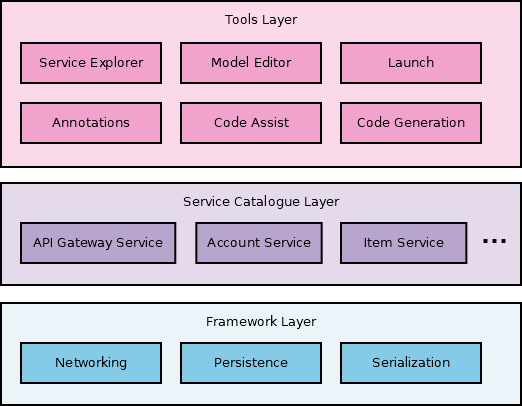
\includegraphics[width=0.7\textwidth]{images/architecture/ArchitectureLayers}
  \caption{The layered architecture of MicroNet with the associated components.}
  \label{fig:architecture_layers}
\end{figure}


The layers and the components they contain are explained below using Component
Responsibility Cards (CRC).

\newpage
\subsubsection{Framework Layer}

The framework layer provides a uniform interface to the core functionality of
MicroNet.\\

\noindent
\begin{tabular}{|l|l|}
    \cline{1-2}
    \multicolumn{2}{|c|}{} \\[-0.3cm]
    \multicolumn{2}{|c|}{Networking Component} \\ 
    \multicolumn{2}{|c|}{} \\[-0.3cm]
    \cline{1-2}
    Responsibility & Collaboration \\
    \cline{1-2}
    & \\[-0.2cm]
    \begin{minipage}{0.47\textwidth}
        \begin{itemize}
          \item Reliable Messaging System
          \item Connection Authentication
          \item Messaging API
        \end{itemize} 
    \end{minipage}
	&
    \begin{minipage}{0.47\textwidth}
        \begin{itemize}
          \item Message Broker (ActiveMQ)
          \item Serialization Component
        \end{itemize} 
    \end{minipage}
	\\ & \\
    \hline
\end{tabular}

\vspace{0.5cm} \noindent 
\begin{tabular}{|l|l|}
    \cline{1-2}
    \multicolumn{2}{|c|}{} \\[-0.3cm]
    \multicolumn{2}{|c|}{Persistence Component} \\ 
    \multicolumn{2}{|c|}{} \\[-0.3cm]
    \cline{1-2}
    Responsibility & Collaboration \\
    \cline{1-2}
    & \\[-0.2cm]
    \begin{minipage}{0.47\textwidth}
        \begin{itemize}
          \item Uniform Database Access
          \item Offer Relational Database 
          \item Offer NoSQL Database
          \item Java API
        \end{itemize} 
    \end{minipage}
	&
    \begin{minipage}{0.47\textwidth}
        \begin{itemize}
          \item Relational DBMS (PostgreSQL)
          \item JDBC
          \item NoSQL Database (Couchbase)
        \end{itemize} 
    \end{minipage}
	\\ & \\
    \hline
\end{tabular}

\vspace{0.5cm} \noindent 
\begin{tabular}{|l|l|}
    \cline{1-2}
    \multicolumn{2}{|c|}{} \\[-0.3cm]
    \multicolumn{2}{|c|}{Serialization Component} \\ 
    \multicolumn{2}{|c|}{} \\[-0.3cm]
    \cline{1-2}
    Responsibility & Collaboration \\
    \cline{1-2}
    & \\[-0.2cm]
    \begin{minipage}{0.47\textwidth}
        \begin{itemize}
          \item Uniform Serialization API
          \item Make serialization technology interchangeable
          \item Json serialization
          \item Binary serialization
        \end{itemize} 
    \end{minipage}
	&
    \begin{minipage}{0.47\textwidth}
        \begin{itemize}
          \item Serialization Library (Gson)
        \end{itemize} 
    \end{minipage}
	\\ & \\
    \hline
\end{tabular}

\subsubsection{Service Catalogue Layer}

The service catalogue was a mainly developed in the second semester thesis
\todo{Chapter 5 Prototype Implementation}. This section will exemplary give
three examples of catalogue services.\\

\noindent
\begin{tabular}{|l|l|}
    \cline{1-2}
    \multicolumn{2}{|c|}{} \\[-0.3cm]
    \multicolumn{2}{|c|}{API Gateway Service} \\ 
    \multicolumn{2}{|c|}{} \\[-0.3cm]
    \cline{1-2}
    Responsibility & Collaboration \\
    \cline{1-2}
    & \\[-0.2cm]
    \begin{minipage}{0.47\textwidth}
        \begin{itemize}
          \item Receive and filter requests from clients
          \item Forward requests to \mss{}
          \item Forward Events to clients
          \item Broadcast events to groups of clients
        \end{itemize} 
    \end{minipage}
	&
    \begin{minipage}{0.47\textwidth}
        \begin{itemize}
          \item Account Service (connection authentication)
        \end{itemize} 
    \end{minipage}
	\\ & \\
    \hline
\end{tabular}

\vspace{0.5cm} \noindent 
\begin{tabular}{|l|l|}
    \cline{1-2}
    \multicolumn{2}{|c|}{} \\[-0.3cm]
    \multicolumn{2}{|c|}{Account Service} \\ 
    \multicolumn{2}{|c|}{} \\[-0.3cm]
    \cline{1-2}
    Responsibility & Collaboration \\
    \cline{1-2}
    & \\[-0.2cm]
    \begin{minipage}{0.47\textwidth}
        \begin{itemize}
          \item User Registration
          \item User Authentication
        \end{itemize} 
    \end{minipage}
	&
    \begin{minipage}{0.47\textwidth}
        \begin{itemize}
          \item Account Database (PostgreSQL)
        \end{itemize} 
    \end{minipage}
	\\ & \\
    \hline
\end{tabular}

\vspace{0.5cm} \noindent 
\begin{tabular}{|l|l|}
    \cline{1-2}
    \multicolumn{2}{|c|}{} \\[-0.3cm]
    \multicolumn{2}{|c|}{Item Service} \\ 
    \multicolumn{2}{|c|}{} \\[-0.3cm]
    \cline{1-2}
    Responsibility & Collaboration \\
    \cline{1-2}
    & \\[-0.2cm]
    \begin{minipage}{0.47\textwidth}
        \begin{itemize}
          \item Player Inventory (Carried Items)
          \item Bank (Item Storage)
        \end{itemize} 
    \end{minipage}
	&
    \begin{minipage}{0.47\textwidth}
        \begin{itemize}
          \item Item Database (PostgreSQL)
        \end{itemize} 
    \end{minipage}
	\\ & \\
    \hline
\end{tabular}

\subsubsection{Tools Layer}

The development of the tool layer was a major part of the lab research. The
tools layer's main purpose is to provide aid with the tenet decentralized
continuous delivery. But the tools layer has also the responsibility to adapt
\ms{} application development to be suitable for \og{} development.\\

\noindent
\begin{tabular}{|l|l|}
    \cline{1-2}
    \multicolumn{2}{|c|}{} \\[-0.3cm]
    \multicolumn{2}{|c|}{Annotation Processing} \\ 
    \multicolumn{2}{|c|}{} \\[-0.3cm]
    \cline{1-2}
    Responsibility & Collaboration \\
    \cline{1-2}
    & \\[-0.2cm]
    \begin{minipage}{0.47\textwidth}
        \begin{itemize}
          \item Framework functionality\footnotemark 
          \item Boilerplate code reduction
          \item Defining the shared messaging API
        \end{itemize} 
    \end{minipage}
	&
    \begin{minipage}{0.47\textwidth}
        \begin{itemize}
          \item Shared Model (to export the API)
        \end{itemize} 
    \end{minipage}
	\\ & \\
    \hline
\end{tabular}

\footnotetext{The user code is
          called by the framework (application skeleton) opposed to the user
          code calling a library (well-defined operations).}
          
\vspace{0.5cm} \noindent      
\begin{tabular}{|l|l|}
    \cline{1-2}
    \multicolumn{2}{|c|}{} \\[-0.3cm]
    \multicolumn{2}{|c|}{Code Assist} \\ 
    \multicolumn{2}{|c|}{} \\[-0.3cm]
    \cline{1-2}
    Responsibility & Collaboration \\
    \cline{1-2}
    & \\[-0.2cm]
    \begin{minipage}{0.47\textwidth}
        \begin{itemize}
          \item Present the Shared API to the developer
          \item Auto-completion of URIs
          \item Recognize API usage errors at compile-time
        \end{itemize} 
    \end{minipage}
	&
    \begin{minipage}{0.47\textwidth}
        \begin{itemize}
          \item Shared Model (to import the API)
        \end{itemize} 
    \end{minipage}
	\\ & \\
    \hline
\end{tabular}

\vspace{0.5cm} \noindent         
\begin{tabular}{|l|l|}
    \cline{1-2}
    \multicolumn{2}{|c|}{} \\[-0.3cm]
    \multicolumn{2}{|c|}{Code Generation} \\ 
    \multicolumn{2}{|c|}{} \\[-0.3cm]
    \cline{1-2}
    Responsibility & Collaboration \\
    \cline{1-2}
    & \\[-0.2cm]
    \begin{minipage}{0.47\textwidth}
        \begin{itemize}
          \item Generate the MicroNet Framework integration classes
          \item Generate POJOs from the Shared Model
        \end{itemize} 
    \end{minipage}
	&
    \begin{minipage}{0.47\textwidth}
        \begin{itemize}
          \item Shared Model (to import the API and Template Types)
          \item Java compiler (annotation processing)
        \end{itemize} 
    \end{minipage}
	\\ & \\
    \hline
\end{tabular}

\vspace{0.5cm} \noindent         
\begin{tabular}{|l|l|}
    \cline{1-2}
    \multicolumn{2}{|c|}{} \\[-0.3cm]
    \multicolumn{2}{|c|}{Service Explorer} \\ 
    \multicolumn{2}{|c|}{} \\[-0.3cm]
    \cline{1-2}
    Responsibility & Collaboration \\
    \cline{1-2}
    & \\[-0.2cm]
    \begin{minipage}{0.47\textwidth}
        \begin{itemize}
          \item Management visual interface for the application (UI)
          \item Compose the application out of catalogue and developed game
          services
        \end{itemize} 
    \end{minipage}
	&
    \begin{minipage}{0.47\textwidth}
        \begin{itemize}
          \item Service Catalogue
          \item Launch Utility (to provide the UI)
        \end{itemize} 
    \end{minipage}
	\\ & \\
    \hline
\end{tabular}

\vspace{0.5cm} \noindent      
\begin{tabular}{|l|l|}
    \cline{1-2}
    \multicolumn{2}{|c|}{} \\[-0.3cm]
    \multicolumn{2}{|c|}{Model Editor} \\ 
    \multicolumn{2}{|c|}{} \\[-0.3cm]
    \cline{1-2}
    Responsibility & Collaboration \\
    \cline{1-2}
    & \\[-0.2cm]
    \begin{minipage}{0.47\textwidth}
        \begin{itemize}
          \item Define and edit the shared model as template types
          \item Instantiate templates as prefabs
          \item Synchronize the Shared Model between developers
        \end{itemize} 
    \end{minipage}
	&
    \begin{minipage}{0.47\textwidth}
        \begin{itemize}
          \item Shared Model (CRUD)
          \item Database Component (for sharing)
        \end{itemize} 
    \end{minipage}
	\\ & \\
    \hline
\end{tabular}

\vspace{0.5cm} \noindent        
\begin{tabular}{|l|l|}
    \cline{1-2}
    \multicolumn{2}{|c|}{} \\[-0.3cm]
    \multicolumn{2}{|c|}{Launch Utility} \\ 
    \multicolumn{2}{|c|}{} \\[-0.3cm]
    \cline{1-2}
    Responsibility & Collaboration \\
    \cline{1-2}
    & \\[-0.2cm]
    \begin{minipage}{0.47\textwidth}
        \begin{itemize}
          	\item Build the composed application
			\item Simplify application deployment
          	\item Provide launch configurations for local deployments 
        \end{itemize} 
    \end{minipage}
	&
    \begin{minipage}{0.47\textwidth}
        \begin{itemize}
          \item Maven (build)
          \item Docker (build \& run)
          \item Docker-compose (compose the application)
          \item optionally uses CDT Launch Groups and Eclipse Docker Tools
        \end{itemize} 
    \end{minipage}
	\\ & \\
    \hline
\end{tabular}

\subsection{Networking}
\label{sub:networking}
Networking in MicroNet has been discussed in detail in section 6.5 Networking
Implementation in project thesis one \cite{biedermann2015project1}. The original
implementation was improved in the course of all three theses and this section
provides a summary of the final implementation solution of networking.

Networking is the most fundamental aspect of an \og{} development and crucial
for the stability of \ms{} applications. The networking concept for \ms{}
applications is heavily influenced by the IDEAL tenet because it makes it
necessary to provide an abstract messaging concept that is decoupled from any
implementation.

In MicroNet this network abstraction is realized by defining a set of networking
capabilities that must be supported by the underlying network technology. These
capabilities are represented in the form of the \code{IPeer} Java interface
shown in \autoref{lst:ipeer_interface}. Standard services can therefore
communicate over an instantiation of the \code{IPeer} interface injected by the
framework. This makes the underlying technology exchangeable since the interface
is stable. This allows platform independence as long as the services are written
in Java.

\begin{figure}
	\begin{lstlisting}[language=Java,firstnumber=1] 
public interface IPeer {
	void startup(URI host);
	void shutdown();
	
	void sendRequest(URI destination, Request request);
	void sendRequest(URI destination, Request request, 
		Consumer<Response> handler);
		
	Response sendRequestBlocking(URI destination, Request request);
	Response sendRequestBlocking(URI destination, Request request,
		int timeout);
		
	void listen(String path, Consumer<Request> handler);
	void listen(String path, Function<Request, Response> handler);
}
	\end{lstlisting}
  	\caption{The iPeer interface must be implemented to participate in MicroNet
  	applications.}
  	\label{lst:ipeer_interface}
\end{figure}

MicroNet implements this networking interface by relying on ActiveMQ as a
message broker. Although it would be possible to replace ActiveMQ as the
MicroNet networking technology this is out of the scope of this thesis to be
validated in practice. As a result MicroNet is heavily dependent on ActiveMQ.

According to the polyglot programming tenet it is a requirement that arbitrary
technologies can participate in a \ms{} application despite the tight coupling
with ActiveMQ. To accomplish this an adapter must be implemented to couple the
foreign technology with the application. The adapter can be an
implementation of an equivalent messaging interface in another programming
language using one of the many proposed ways to integrate with ActiveMQ like
RESTful HTTP, JMS, .NET, C/C++, Go, Node.js, Python, and more.

For game engine integration the messaging interface also has to be implemented
in the respective technology of the engine. In the case of MicroNet ActiveMQ
Unity3D is used as the refernce game engine which is written in C\#. For this
purpose the NMS \gls{api} which is a .NET port of the Java Message Service (JMS)
interface is used to make MicroNet accessible from the Unity3D game engine.

\subsubsection{Messaging System}

Messaging in MicroNet evolves around patterns: API Gateway, Reverse Proxy and
Pipes and Filters.

MicroNet uses a reverse proxy to interchange messages from the public Internet
with the internal network used by MicroNet. For this purpose two separate
message brokers are used and only the public broker is exposed to the Internet.
The gateway intercepts all messages from the public network and forwards them to
the responsible \ms{}. This is further detailed in the Messaging \gls{api} section
below.

The reverse proxy in fact also is the API gateway. An API gateway is a standard
approach offering the \textit{Service API} to the users. Upon reception of a
message the gateway can filter it according to a white- or blacklisting approach.

\begin{figure}
\begin{lstlisting}[language=Java,firstnumber=1] 
@MessageService(uri = "mn://foo")
public class ServiceFoo {
	@OnStart
	public void onStart(Context context) {
		URI destination = URI.create("mn://bar/hello");
		Request request = new Request("Hello from Foo!");
		context.getPeer().sendRequest(destination, request, response -> {
			System.out.println("Received Response: " + response.getData());
		});
	}
}

@MessageService(uri = "mn://bar")
public class ServiceBar {
	@MessageListener(uri="/hello")
	public Response helloHandler(Context context, Request request) {
		System.out.println("Received Request: " + request.getData());
		return new Response(StatusCode.OK, "Likewise, Bar");
	}
}
\end{lstlisting}
\caption{Two MicroNet services communicating with each other.}
\label{lst:service_communication}
\end{figure}

\mss{} can access the messaging functionality by using the context object
injected by the framework. \autoref{lst:service_communication} shows an example
of two simple \mss{} communicating with each other. It has to be mentioned that
the two services in the listing are fully functional without any additional
code necessary. The setup of the context and the \ms{}'s main function are
completely abstracted by the framework.

\paragraph{Message Parameters}

One useful feature that MicroNet provides are typed message parameters. These
parameters are defined using Parameter Codes and the \textit{Template Types}
both defined int the \textit{Shared Model}.

Message parameters spare the developer the need to individually define a
specific payload for each message transfer. For example slightly different
messages can be distinguished by only using parameter codes and leaving the
payload unchanged.

\begin{figure}
\begin{lstlisting}[language=Java,firstnumber=1] 
@MessageService(uri = "mn://foo")
public class ServiceFoo {
	@OnStart
	public void onStart(Context context) {
		URI destination = URI.create("mn://bar/hello");
		Request request = new Request("Hello from Foo!");
		request.getParameters().set(ParameterCode.ID, 42);
		context.getPeer().sendRequest(destination, request);
	}
}

@MessageService(uri = "mn://bar")
public class ServiceBar {
	@MessageListener(uri="/hello")
	public void helloHandler(Context context, Request request) {
		int parameter = request.getParameters().getInt(ParameterCode.ID);
		System.out.println("Received Request with Parameter: " + parameter);
	}
}
\end{lstlisting}
\caption{Adding a parameter to a MicroNet message.}
\label{lst:message_parameters}
\end{figure}

\autoref{lst:message_parameters} shows how services can transmit parameters
along with a request. For responses this works exactly the same.

\subsubsection{Connection Authentication}

Security is always a concern in regard to Internet applications. The backbone
of distributed application security is user connection authentication.
Since multiple gateways can be active simultaneously the integrity of the user
has to be validated by the gateway with every request. The gateway validates the
user request by looking up the user connection in the session store and
comparing it to the connection the request was received from. If no user session
is present in the session store the user connection is considered
unauthenticated.

For unauthenticated connections the gateway only forwards login messages to the
login service. Upon a positive login response from the account service the
processing gateway adds the user connection to the session store. Other gateways
are then able to look up if a connection is authenticated. The advantage of this
solution is that it scales very well. The downside is that it involves many
reads of the session store.

A requirement for this approach to work is that the underlying networking
provides a way to correlate incoming messages with a connection. This can be
done generating a connection ID hash based upon the user's IP/port combination.
ActiveMQ has this capability already built in by providing a globally unique
connection ID per connection.

The connection authentication process is further explained in
\autoref{sub:session_management}.

\subsubsection{MicroNet Messaging API}

The messaging \gls{api} provided by a MicroNet applications is a direct implementation
of the fine-grained interfaces tenet. It offers the following functionality to
promote stateless message transfers:

\begin{itemize}
  \item Sending a request to a \ms{} either from a user or another \ms{}
  \item Sending a request to a \ms{} and waiting for a response with a
  short\footnote{5 - 15 seconds of timeout seem appropriate for most short
  requests.} timeout either from a user or another \ms{}
  \item Sending an event to a user from a \ms{}
  \item Sending an event to a group of users from a \ms{}
  \item Sending a message to a topic, meaning to all subscribed \mss{}
  \item Named message parameters
\end{itemize}

\begin{figure}
	\centering
	\hspace*{-1.5cm}
	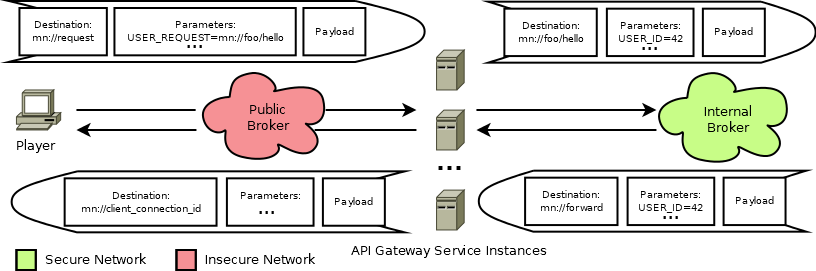
\includegraphics[width=1.2\textwidth]{images/architecture/MessagingAPI}
	\caption{The API Gateway offers the MicroNet messaging \gls{api} to the player.}
	\label{fig:messaging_api}
\end{figure}

These messaging capabilities are sufficient to model any arbitrary message
transfer. They leave a great degree of freedom and make message transfer
implementation very comfortable. 

\autoref{fig:messaging_api} shows the communication between a user and a
MicroNet application. The user in this scenario is already authenticated so the
gateway only needs filter client quests according to access restrictions. The
user sends his request to the \code{mn://request} queue which leads to an
arbitrary gateway instance consuming the request. The gateway reads the
\code{USER\_REQUEST} parameter from the request and according to it forwards the
message to the internal broker. Depending on the situation if the user expects a
response within the defined timeout or if no response is expected the
gateway holds on to a temporary response queue which allows immediate responses.
Such an immediate response can also indicate that the request will need longer
to be processed and therefore the requestor has to act accordingly and wait for
an asynchronous response.

These asynchronous responses are called events. An event can either be sent to a
single user or to a group of users. For this purpose \mss{} can send a request
to the \code{mn://forward} queue which is consumed by any gateway who in
response forwards the event to the corresponding user or group.

One last feature of the MicroNet messaging \gls{api} is the ability to send messages
to topics which can be subscribed by any service. This allows services to react
on events happening throughout the application. This can be for example the
\textit{new player connected} event.












\subsection{Composition Concepts}

The major challenge during the development of a \ms{} application is to achieve
loose coupling according to the IDEAL tenet. The goal of loose coupling is to
reduce dependencies among services. It has to be noticed that the coupling
between services can never be zero. Without any coupling the application cannot
function as a whole. MicroNet several basic concepts to reduce service coupling
while preserving reasonable development comfort. These concepts are discussed in
this section.

\subsubsection{Dependency Abstraction}

Dependency abstraction is a concept to reduce the number of dependencies
that \mss{} must explicitly add to the Java classpath to access core
functionality networking, persistence, and serialization.

According to the dependency abstraction concept external libraries are wrapped
within the core framework to offer standard access to the underlying dependency.
\mss{} can use the MicroNet wrapper libraries instead of using the
dependencies directly. This allows for exchangeability of the dependencies
without touching any \mss{} services. MicroNet integrates dependent libraries
into the wrapper libraries by the use of Maven which allows a very flexible
dependency chain. \autoref{fig:dependency_abstraction} shows which libraries are
abstracted by which framework component.

\begin{figure}
	\centering
	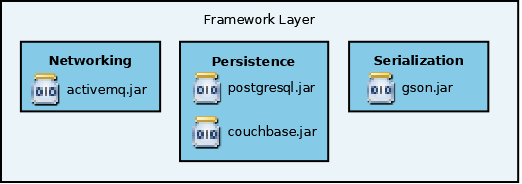
\includegraphics[width=10cm]{images/architecture/DependencyAbstraction}
	\caption{Dependency Abstraction in the MicroNet core framework.}
	\label{fig:dependency_abstraction}
\end{figure}

It has to be mentioned that the dependency abstraction layer is a dependency
itself and therefore it increases service coupling. But since the abstraction
layer unifies dependency access it helps to respect the don't repeat yourself (DRY)
principle and therefore increases overall cohesion of the application. 

Since the MicroNet adaption layer is realized using Java wrapper libraries,
this approach works very well for all Java \mss{} but none Java services have to
use the dependencies directly.

\subsubsection{Shared Model}
\label{subsub:shared_model}

The general design of how to incorporate a game model into a \mn{} application
is reclined to the design of modern game engines like Unity3D or UnrealEngine 4.
What these engines have in common is a graph to store the game state e.g. all
objects, levels, players, etc. This concept of game data organization will be
referred as the game graph. Two examples of game graphs are shown in
\autoref{fig:scenegraph}.

\begin{figure}
  \centering
  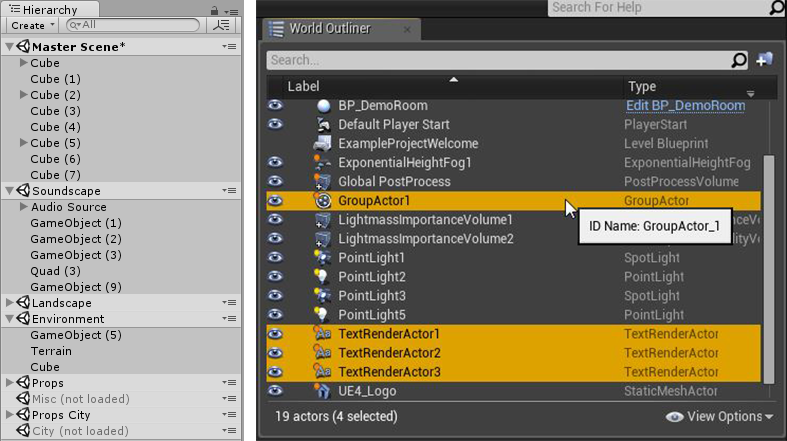
\includegraphics[width=\textwidth]{images/game_engine/scenegraph}
  \caption{Two example game graphs of the Unity3D (left) and the UnrealEngine4
  (right).}
  \label{fig:scenegraph}
\end{figure}

The shared model concept is mainly inspired by game graph concept of game
engines. The graph is represented by a Json document structure and can be shared
either using a git repository or by using a development database. The Json
format helps to achieve platform independence.

The shared model specifically allows to strongly type message transfers and
unifies database access. The design of the shared model allows to integrate the
game graph in a game engine because the concepts are closely related.

The shard model represents the game graph in the form of two individual trees:
The template tree and the prefab tree. The template tree is responsible to store
types. Types are templates to define all entities of the game. Entities are not
restricted to one purpose and can be used to store or transmit domain data.
Templates are plain data objects and can be thought as the equivalent to Java
POJOs. Momentarily it is not possible to add game logic to templates. But this
is planned for the future by using code injection (explained in
\autoref{sub:model_code_injection}). \autoref{lst:template_type} shows an
example of a template type in the template tree.

The types supported of the template tree are directly derived by the java types
because they work natively with the Java side of MicroNet. The Java types are
well documented in the Java language definition and can therefore be replicated
in other programming language to achieve deterministic behaviour on all systems.
The supported types are: STRING, NUMBER (INT, FLOAT, DOUBLE, \ldots), BOOLEAN, CHAR,
ENUM, LIST, SET, MAP, and COMPONENT. More information about the supported types
can be found in paragraph Model Editor in \autoref{sub:tools}.

\begin{figure}
\begin{lstlisting}[language=json,firstnumber=1] 
{
  "name": "UserValues",
  "variables": [
    {
      "name": "id",
      "type": {
        "numberType": "INT",
        "type": "NUMBER"
      }
    },
    {
      "name": "credentials",
      "type": {
        "componentType": "CredentialValues",
        "type": "COMPONENT"
      }
    }
  ]
}
\end{lstlisting}
\caption{The template type for the UserValues domain object in the template
tree.}
\label{lst:template_type}
\end{figure}

The second tree is the prefab tree. It is responsible to store actual instances
of templates representing the statical part of the game state. The prefab tree
is a concept to allow game designers to define the properties of the game in a
way which is directly understood by MicroNet and can therefore directly be used
to persist and synchronize the game. \autoref{lst:prefab_type} shows how a
prefab of the \code{UserValues} object looks like.

\begin{figure}
\begin{lstlisting}[language=json,firstnumber=1] 
{
  "id": 42,
  "credentials": {
    "username": "Jonas",
    "password": "1234"
  }
}
\end{lstlisting}
\caption{A prefab of the UserValues template type.}
\label{lst:prefab_type}
\end{figure}



\subsubsection{Service API}

The messaging system described in \autoref{sub:networking} is the main driver
for logical composition in MicroNet applications. The service API is offered to
the user by the API gateway in the form of a URI addressing. \mss{} can also use
this scheme to find each other internally. The only requirement to use the API
is to have access to the underlying message broker either trough the MicroNet
networking component or a direct connection to ActiveMQ.

The MicroNet service API is defined by using static URIs using the specific
form: \textit{ms://servicename/fine/grained/api}. The host portion of the URI is
used for participant discovery by using the message broker functionality to
register queues for the specific service address, \textit{ms://servicename} in
this example. The remainder of the URI, \textit{fine/grained/api} in this
example represents the fine grained service API defined by the \ms{} according
to tenet Fine-grained Interfaces. This Service API scheme of MicroNet is
inspired by a RESTful URI schema but is only static\footnote{Requests to URIs
like \textit{mn://player/123341214/some/functionality} are not realized}. Within
\mss{} the service API is defined using Java annotations described in paragraph
Annotations in \autoref{sub:tools}.

\subsubsection{Service Catalogue}

The service catalogue is a layer of MicroNet that uses the underlying framework
to provide reference service implementations for commonly requires
functionality. The service catalogue is realized by using Maven archetypes. An
archetype represents a skeleton or a basic implementation of a feature and can
be extended by the developer. It is possible for developers to contribute
services to a private service catalogue by creating a new Maven archetypes and
making them available for future reuse. \autoref{fig:service_catalogue} shows
how the service catalogue is integrated in the game development process.

\begin{figure}
	\centering
	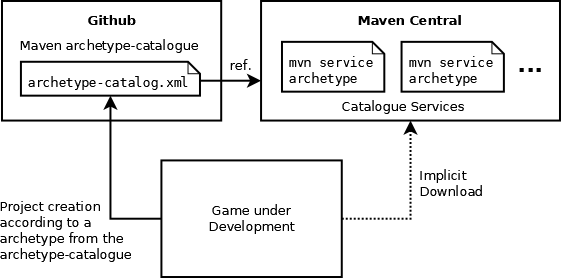
\includegraphics[width=12cm]{images/architecture/ServiceCatalogue}
	\caption{Integration of the service catalogue in \og{} development.}
	\label{fig:service_catalogue}
\end{figure}

The mostly used \ms{} of the service catalogue is the ``Hello World''
service which provides the means of bringing up a new \ms{} quickly.

\subsubsection{Consistency Requirements}

Consistency is a big concern in any distributed application and \ogs{} are no
exception. Consistency requirements for \ogs{} has already been researched in
project thesis one \todo{5.4 Non-functional requirements} and have been further
examined in this semester.

For \ogs{} consistency requirements can be categorized into strong consistency
for sensitive data like account or payment information and eventual consistency
for all other non critical game data. 

The final solution to consistency in MicroNet emphasises exactly this two
requirements. For transaction which require strong consistency it is aways
necessary that one single \ms{} maintains the overall control over the complete
transaction. This service then must use the underlying relational database to
make the transaction ACID by using the two phase commit protocol offered by the
database which is ProstgreSQL for MicroNet. This approach is mainly chosen due
to the reason that ACID transaction using eventual consistency are hard to get
right and therefore are error-prone \cite{zhang2011transaction},
\cite{zhang2008persistence}, and \cite{pardon2014atomic}.

For best effort consistency requirements eventual consistency is a solution that
has proven to work \cite{graham2016distributed_transactions}. Eventual
consistency emphasis scaling and robust systems in general. The drawback is the
added effort during development to implement a eventual consistent application.

Eventual consistency in MicroNet is realized by time-outs and retries. This is
realized by using the presistence system of the message broker in conjunction
with the request response functionality offered by MicroNet messaging. \mss{}
are advised to retry a transaction for a number of times\footnote{Five retries
seemed appropriate for most requests.}. If all retries where failures the
service must persistently log the unprocessed transaction and send an
informative message to the user. Over time the number of unprocessed transaction
should decrease. Unprocessed transaction can then be examined by developers in a
batch to find flaws in the application design.
developers

\subsection{Session Management}

MicroNet provides session management as a high level feature to tackle the
integral part of session handling in a \og{}. Player sessions are essential to
track actions of individual players and persist the progress of a player. Game
sessions tackle the issue that \ogs{} are state-full and therefore game session
in simulation services are unique. 

Session management has been one major issue throughout thesis one, two and
three. The final solution for session management relies on a NoSQL database.




\subsubsection{Player Sessions}

The authentication process that has briefly been mentioned in
\autoref{sub:networking} is responsible to establish player sessions. Once
authenticated player sessions can be used to collate incoming messages to users.
Player sessions can also be used to store frequently changing player data to
allow fast and global access. In MicroNet the player sessions can be accessed
through Couchbase.

One drawback that player session introduce is the fact that multiple API
gateways each gateway needs the ability to look-up player connections to
determine if the corresponding user is authenticated. This process has to be
done upon every player message which leads a lot of access to NoSQL. Another
possibility would be that the user needs to send a authentication cookie with
every message. This method introduces significant bandwidth overhead which is
worse. 

\begin{figure}
	\centering
  	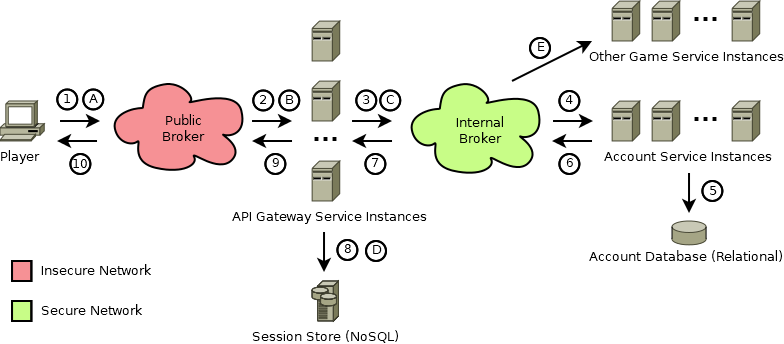
\includegraphics[width=\textwidth]{images/architecture/PlayerSessions}
	\caption{Player session authentication process.}
	\label{fig:player_sessions}
\end{figure}

\autoref{fig:player_sessions} shows the whole authentication process with the
result of a established authenticated player connection. The message flow
consists of the following steps:

\begin{enumerate}
  \item The user sends a login request to the public broker.
  \item One API Gateway polls the message in a competing consumer fashion.
  \item The gateway forwards the login message to the internal broker using the
  mn://account/login queue.
  \item One Account Service polls the message in a competing consumer fashion.
  \item The Account Service authenticates the user using the Account Database.
  \item The account service returns the login response to a temporary queue held
  open by the responsible gateway.
  \item The gateway service consumes the login response from the temporary
  queue.
  \item Upon login success the gateway adds a new player session to the session
  store, identified by the player connection.
  \item The gateway returns the login response to a temporary queue held open by
  the requesting player.
  \item The player consumes the login response from a temporary queue. Upon
  success he gains access to the game services (A, B, C, D\footnote{In step D
  the API Gateway must verify if the player connection is already
  authenticated. If the player is not authenticated no messages are forwarded.},
  E).
\end{enumerate}



\subsubsection{Game Sessions}

Game sessions are a strategy to deal with the state-fullness of \ogs{}. Game
sessions are unique and a player can only be in one game session at a time. Game
sessions are either infinitely or terminate at specific conditions. Either way
the player must be able to find the correct simulation instance which hosts the
game session he wants to participate in. MicroNet provides this functionality
through the WorldService which is part of the service catalogue.

\begin{figure}
	\centering
  	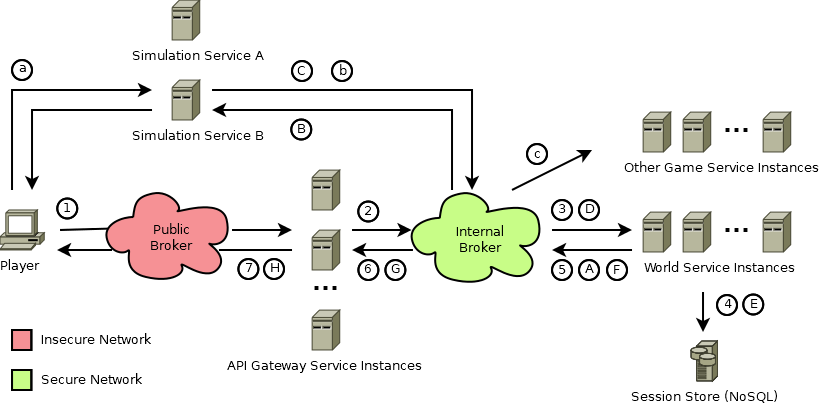
\includegraphics[width=\textwidth]{images/architecture/GameSessions}
	\caption{The join process of a game session.}
	\label{fig:game_sessions}
\end{figure}

\autoref{fig:game_sessions} shows the process how a game session is joined.
The join process consists of the following steps:

\begin{enumerate}
  \item The player sends a join request for game session B to the API gateway
  via the public message broker.
  \item The gateway service forwards the message to the mn://world/join queue
  via the internal message broker.
  \item One world service polls the message in a competing consumer fashion
  \item The world service checks is the session already exists in the session
  store. If not, the world service adds the game session to the session store,
  marks it as \textit{isOpening} and initiates the game session opening process (capital
  letter sequence in \autoref{fig:game_sessions}). In this case or if the
  session is currently opening the world service adds the player to a waiting
  queue for the session.
  \item If the game session is open the world service directly
  forwards the IP/Port combination to the player.  In this case the session is
  not open or opening a ``please wait'' response is forwarded to the player.
  \item The join response is consumed by a temporary queue held open by the API
  Gateway. The gateway forwards the join response to the player via the public
  broker.
  \item The player consumes the join response using a temporary queue. In the
  case the session was already open, the player can join right away. The regular
  session flow (a, c, c, \ldots) starts now.
\end{enumerate}

In the case the requested game session is not open when the player wants to
join\footnote{It is a common case that the game session is not open, for
example when the \og{} has many (thousands) of available game sessions.} the
session must be started asynchronously and the player must be notified when the
session is ready. This process consists of the following steps:



\begin{enumerate}[label=\Alph*.]
    \item The World Service sends an open region request to the
    mn://instance-open queue.
    \item One free simulation instance polls the open request in a competing
    consumer fasion.
    \item Once the simulation service is up and running, sends a simulation
    instance ready to the mn://world/instance/ready queue via the internal
    message broker.
    \item One World Service polls the instance ready message in a competing
    consumer fashion.
    \item The World Service marks the game session as \textit{isOpen} in the
    session store.
    \item The World service sends a broadcast event request to the
    mn://gateway/broadcast/event queue containing the IP/Port combination of the
    simulation service, addressed to all player is the waiting queue of the game
    session.
    \item One API Gateway polls the broadcast requests in a competing consumer
    fashion
    \item The Gateway broadcasts the join event to all waiting players. From
    then on the regular session flow (a, c, c, \ldots) starts.
\end{enumerate}





\subsection{MicroNet Tools}
\label{sub:tools}

The MicroNet tools are a collection of Eclipse plug-ins. Eclipse was chosen due
to the primary Java nature of MicroNet. This allows a quick development of Java
\mss{}. But the MicroNet tools also offer a way to integrate other
technologies into a \ms{} application. This language independence is
accomplished by using \gls{json} as a low level information exchange format. As
long as a technology supports \gls{json} it can participate in the application.
Another requirement is that it is possible to access to the message broker with
the foreign technology.

Since the \gls{ui} of an Eclipse plug-in is written using the Swing
Window Toolkit (SWT) library it can easily be exported to be a stand-alone tool
decoupled from Eclipse. With this approach it is possible to port the MicroNet
Tools to other platforms as long as they support a \gls{jvm}.

The MicroNet Tools have been completely developed within this last semester
thesis and are a major contribution to four of the hypotheses listed in
\autoref{sub:hypothesis}: the composition, deployment, simple development, and 
reproducibility hypotheses.

More information on the MicroNet Tools can be found in the MicroNet online
documentation \cite{micronet2017doku}.

\subsubsection{Files and Folders Structure}

To allow loose coupling of a \ms{} application MicroNet makes a few assumptions
on how to organize files and folders:

\begin{itemize}
  \item The eclipse workspace folder must contain one project folder for each
  \ms{}.
  \item For automated integration of a \ms{} its project folder must be either a
  Java/Maven project or it must contain a Dockerfile.
 \item One shared folder must be present to exchange the \textit{Shared Model} and the
  \textit{Service API}.
\end{itemize}  

\begin{figure}
	\centering
	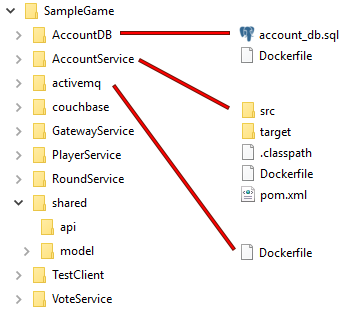
\includegraphics[width=9cm]{images/tools/folder_structure}
	\caption{Example folder structure of a MicroNet application workspace.}
	\label{fig:folder_structure}
\end{figure}

\autoref{fig:folder_structure} shows an example of a folder structure of a
MicroNet application workspace. The shared folder in this case is simply a folder within the
workspace. The figure also shows three canonical examples of project folders.
The AccountDB folder represents a containerized PostgreSQL database. The
AccountService folder is a standard MicroNet Maven/Java service project. The
activemq folder contains only a Dockerfile, which is the minimal requirement to
participate in a MicroNet application.

\subsubsection{Annotations}

MicroNet \textit{Annotations} provide a solution to define a \ms{} in a very
lean way. A service is defined by annotating an arbitrary class in the service
projects with the \textit{@MessageService(uri=``mn://service\_name'')}
\textit{Annotation}. Within the service class listener methods can be annotated
with the \textit{@MessageListener(uri=``/api\_method'')} \textit{Annotation} to
define the reactive behaviour of the service according to the defined \gls{api}.
Examples of services defined by the \textit{Annotation} can be seen in
\autoref{lst:service_communication} and \autoref{lst:message_parameters}.

\begin{figure}
\begin{lstlisting}[language=Java,firstnumber=1] 
@MessageService(uri = "mn://foo")
public class ServiceFoo {
	@OnStart
	public void onStart(Context context) {
		System.out.println("Start called");
	}
	
	@OnStop
	public void onStop(Context context) {
		System.out.println("Stop called");
	}
	
	@MessageListener(uri="/hello")
	@RequestPayload(UserValues.class) 
	@ResponsePayload(CredentialValues.class)
	@RequestParameters({
		@MessageParameter(code=ParameterCode.ID, type=Integer.class),
		@MessageParameter(code=ParameterCode.NAME, type=String.class)
	})
	@ResponseParameters({
		@MessageParameter(code=ParameterCode.ID, type=Integer.class),
	})
	public Response helloHandler(Context context, Request request) {
		int idParameter = request.getParameters().getInt(ParameterCode.ID);
		String nameParameter = request.getParameters()
			.getString(ParameterCode.NAME);
		
		UserValues user = Serialization.deserialize(
			request.getData(), UserValues.class);
		System.out.println("Process: " + user + " and " + nameParameter);

		String responseData = Serialization.serialize(user.getCredentials());
		Response response = new Response(StatusCode.OK, responseData);
		response.getParameters().set(ParameterCode.ID, idParameter);
		return response;
	}
}
\end{lstlisting}
\caption{A fully defined MicroNet \ms{} including all possible pre- and
post-condition \textit{Annotations}.}
\label{lst:pre_post_conditions}
\end{figure}

MicroNet \textit{Annotations} also provide a basic implementation of the design
by contract pattern. A service defines preconditions on request payloads and
defines post-conditions on response payloads. This system aims to prevent
semantic errors in communications. The pre- and post-conditions build the
foundation of the \textit{Code Assist} tool of MicroNet which helps the
developer in preventing mistakes in \ms{} communication design.
\autoref{lst:pre_post_conditions} shows a \ms{} defined by \textit{Annotations}
containing a well defined message listener with all pre- and post-conditions.
Theoretically the \textit{@RequestParameter} and \textit{@ResponseParameter}
\textit{Annotations} could implicitly be generated by parsing the \gls{ast} of
the listener method. This is however a very advanced topic which could fill a
whole thesis in itself.
 
 \paragraph{Annotation Processing}
 
Java annotations can either be used during run-time or processed during
compilation-time. MicroNet only processes \textit{Annotations} at compile-time.
Since Java version 6 the annotation processing process is tightly integrated
into the standard Java build process. This renders the \textit{Annotation}
process platform independent and it can be reproduced in a command line java
build, a Maven build or an Eclipse build\footnote{Annotation processing is
executed by the Java compiler which behaves slightly different for all evaluated
build setups (Eclipse, Maven, or Java native). Specifically newly generated
annotations are only found by the Eclipse proprietary compiler.}.

\textit{Annotation Processing} is also the entry point for code generation.
Even if no annotations are present in a project \textit{Annotation Processing}
can still be activated just to generate the \textit{Shared Model} and without
generating any service implementation. The MicroNet \textit{Annotation
Processor} provides an option for this purpose.

\subsubsection{Code Generation}

Code generation allows the developer to omit the boiler plate code that is
needed to integrate a service into a MicroNet application. This covers the setup
of the appropriate networking solution according to the environment and the
generation of the executable class of the \ms{}. This simplification allows the
developer to focus more on the actual domain logic of the \ms{}. It also spares
the developer having to register the main service class within the
application. The service class is automatically found and registration is
implicitly done by the \textit{Annotation Processor}.

The code generation library of MicroNet is very small and can be translated to
other programming languages very easily if needed. Since code generation is
basically nothing more than generating the right ``text-files'' this can be
accomplished in almost any imaginable programming language.

The MicroNet code generation library is implemented using the Java Poet
library. Java Poet allows for typesafe generation of Java classes and is very
easy to use. 

\paragraph{Service Generation}

The \textit{@MessageService} and \textit{@MessageListener} \textit{Annotations}
are used to build the executable class of a \ms{}. The executable class
registers all message listeners within the networking system. In addition the
annotated \textit{@Start} and \textit{@Stop} methods are called at service start
or at service termination respectively. The generated main method encompasses
the start/stop functionality and the listener registration in a defined set-up
sequence. \autoref{lst:generated_service} shows the generated implementation of
the annotated service shown in \autoref{lst:pre_post_conditions}.

\begin{figure}
\begin{lstlisting}[language=Java,firstnumber=1] 
public final class ServiceImpl {
  public static void main(String[] args) {
    try {
      System.out.println("Starting ServiceFoo...");

      IPeer peer = PeerFactory.createPeer();
      Context context = new Context(peer, "mn://foo");
      ServiceFoo service = new ServiceFoo();

      System.out.println("Registering message listeners...");
      peer.listen("/hello", (Request request) -> 
      	service.helloHandler(context, request));

      System.out.println("ServiceFoo started...");
      service.onStart(context);

      Runtime.getRuntime().addShutdownHook(new Thread() {
        @Override
        public void run() {
          System.out.println("ServiceFoo stopped...");
          service.onStop(context);
        }
      });
    }
    catch (Exception e) {
      System.err.println("Could not start ServiceFoo...");
      e.printStackTrace();
    }
  }
}
\end{lstlisting}
\caption{An executable \ms{} main class generated out of an annotated service
class.}
\label{lst:generated_service}
\end{figure}

\paragraph{Model Generation}

The model generation process is completely independent from the service
generation and is used to translate the game model which is defined in
\gls{json} to java POJOs (plain old Java objects). Because the MicroNet Model
generation library is very small it can also be reproduced in other programming
languages with relative ease. \autoref{lst:generated_model_class} shows the
\textit{UserValues} POJO generated out of the corresponding \textit{Template Type}
shown in \autoref{lst:template_type}.

\begin{figure}
\begin{lstlisting}[language=Java,firstnumber=1] 
public class UserValues {
  private int id;
  private CredentialValues credentials;

  public void setId(int id) {
    this.id=id;
  }

  public int getId() {
    return id;
  }

  public void setCredentials(CredentialValues credentials) {
    this.credentials=credentials;
  }

  public CredentialValues getCredentials() {
    return credentials;
  }
}
\end{lstlisting}
\caption{The UserValues POJO created out of the corresponding \textit{Template Type}.}
\label{lst:generated_model_class}
\end{figure}

The challenge for model generation is not the generation process itself but the
definition and editing process of the model that is generated and its
representation. These aspects make up a much larger part of MicroNet than the
actual code generation. Model editing and representation is further discussed
below in the paragraph on the \textit{Model Editor}.

\subsubsection{Code Assist}

The \textit{Code Assist} plug-in helps the developer to keep track of
functionality provided by other services. It presents the \textit{Service API}
in a type-safe way to the developer by relying on the pre- and postconditions
defined by MicroNet \textit{Annotations}.

\textit{Code Assist} is implemented by using the Eclipse code-completion
extension point. This extension point is used to add custom entries to the code
completion list box. This functionality is used to offer the MicroNet \gls{api}
to the developer any time he types \textit{``mn://''} in a source file. The
proposals are filtered according to the developer's input.

Type-safety enforcement is currently not implemented in MicroNet due to the same
reason as mentioned above in the section on \textit{Annotations} that require
parsing the \ms{} code. It could however be implemented by searching the
\gls{ast} of a message handler method for references on the request and response
objects. Calls to \code{getParameters()} or \code{setParameters()} can be
analyzed in regard to which \code{ParameterCode}s are used and which the
\textit{Template Type} of the parameter is. This feature would allow the
developer to omit the \code{@RequestParameters} and \code{@ResponseParameters}
\textit{Annotations}.

Upon violation of the message types the compiler can generate an error which
forces the developer to fix the issue before a build can be executed.
Although this process is possible the implementation of violation detection
again involves parsing the Java \gls{ast} and this effort is out of the scope of
this thesis.

In the current version of MicroNet the types are presented to the developer via
a tool-tip. Although type-safety is not enforced the developer can at least read
the correct types in the \textit{Code Assist} tool-tip, which alone is already
very helpful. \autoref{fig:code_assist} shows the \textit{Code Assist} tool-tip
for the \code{mn://foo/hello} message listener that was shown in 
\autoref{lst:pre_post_conditions}.

\begin{figure}
	\centering
	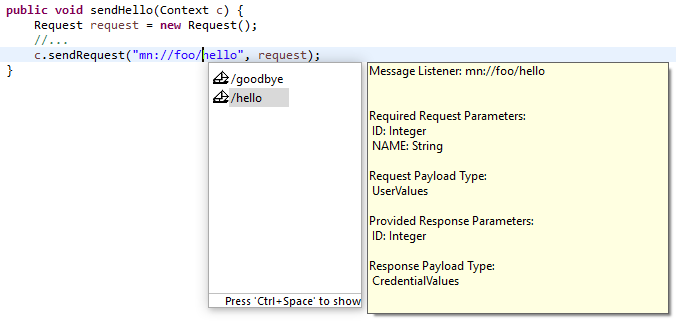
\includegraphics[width=\textwidth]{images/tools/CodeAssist}
	\caption{MicroNet \textit{Code Assist} tool-tip.}
	\label{fig:code_assist}
\end{figure}

\subsubsection{Service Explorer}

The \textit{Service Explorer} is the central management UI of a MicroNet and
helps the developer to get an overview over the whole game application. The
\textit{Service Explorer} is realized using a custom Eclipse view. The view
contains a list of all services showing their versions along with other useful
information like required ports or links to other services. The \textit{Service
Explorer} displays services which are Java, Maven and Docker projects. The
service list is dynamic and automatically refreshed when projects are created or
deleted.

The service list can be used to quickly edit the configuration of services. This
includes the port configuration as well as service linkage for the Docker
overlay network.

The \textit{Service Explorer} is also used to configure the composition of the
application in a visual way. Services can be activated to be part of the build
process, which automatically integrates them into the composition files (Maven:
pom.xml, Docker: docker-compose). This is done by deciding for each service
individually if it is part of the Maven build and/or part of the Docker
container build process.

The \textit{Service Explorer} also provides a quick interface to all launch
configurations explained in the \textit{Launch Utility} section below. The launch
functionality is provided with a context menu for each service in the list and
through the local pull-down menu offered by the Eclipse view.
\autoref{fig:service_explorer} shows the \textit{Service Explorer} with the
launch menu of the \code{FooService} open.

\begin{figure}
	\centering
	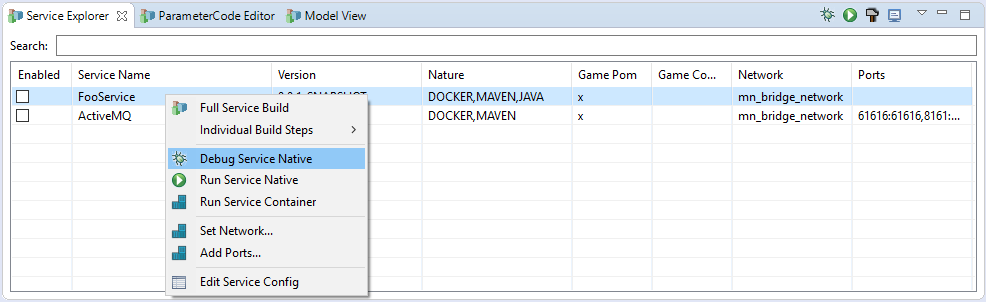
\includegraphics[width=\textwidth]{images/tools/ServiceExplorer}
	\caption{MicroNet \textit{Service Explorer}}
	\label{fig:service_explorer}
\end{figure}

\subsubsection{Launch Utility}

The \textit{Launch Utility} brings order to the vast different possibilities of
how to orchestrate a \ms{} application with containers. Many different configurations
can be helpful to develop, test and deploy a \ms{} application. The MicroNet
launch tools provide an easy way to set-up and start launch configurations.

The launch configurations of a Java/Maven build are offered via the Eclipse
Launcher plug-in. For these configurations the MicroNet \textit{Launch Utility}
only has to run the respective Eclipse Launch configuration.

Automation of the Docker container build process is not as simple because
Eclipse does not offer built-in functionality to access the Docker daemon.
The Docker Tools for Eclipse can be used to fulfill this gap since it provides
the necessary Docker container launch configurations. This however introduces a
strong dependency on the Docker Tools, which is undesirable. Many client for the
Docker daemon exist to integrate Docker automation into applications. This
however introduces another dependency closely related to Eclipse; and also the
tested Spotify Docker client which looks very promising has caused several class
path run-time errors and does not support Docker compose.

A workaround is to automate the Docker CLI using the Java run-time environment.
With this approach the docker commands are simply executed on the host of the
\gls{jvm}. This decouples the Docker integration mainly from Eclipse and places
it into the used Docker CLI. A Docker CLI is available for all major platforms:
Linux, Windows and MacOS. Since the docker CLI commands are the same on all
systems this is a platform independent approach since it only relies on a
\gls{jvm} and the docker CLI which is installed alongside Docker anyway. A
Drawback is that the developer has to configure the host-path to the docker CLI
executables. This is further complicated when Docker Toolbox instead of native
Docker is used since Docker Toolbox requires setting several Docker environment
variables. The MicroNet \textit{Launch Utility} however encompasses all this
functionality.

The \textit{Launch Utility} can deploy MicroNet applications in three distinct ways which
can all be combined which each other: local native, local containerized, and
cloud containerized. \autoref{fig:launch_utility} shows how the launch
configurations can be started via the \textit{Service Explorer}. The rest of this
paragraph explains all three deployment modes.

\begin{figure}
	\centering
	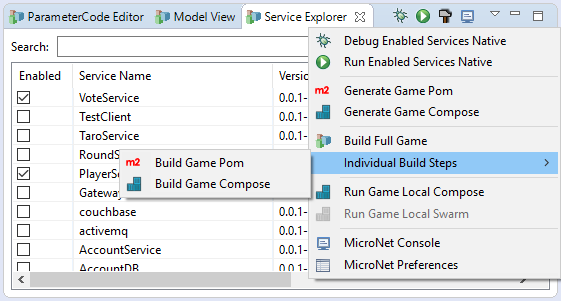
\includegraphics[width=14cm]{images/tools/LaunchUtility}
	\caption{\textit{Launch Utilities} offered by the \textit{Service Explorer}}
	\label{fig:launch_utility}
\end{figure}

\paragraph{Local Native}

\begin{figure}
	\centering
	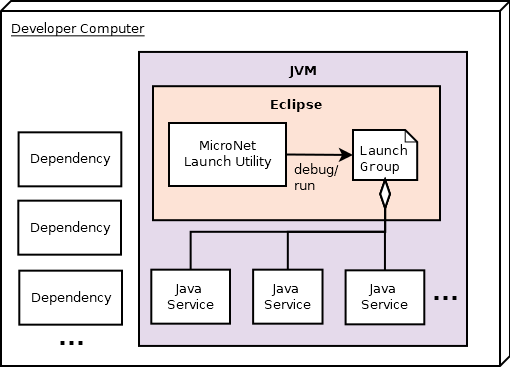
\includegraphics[width=10cm]{images/architecture/DeploymentLocalNative}
	\caption{Local native deployment of a MicroNet driven application.}
	\label{fig:deployment_local_native}
\end{figure}

The native configuration runs or debugs a game application as a set of native
Java applications. This makes debugging very fast and the integration in Eclipse
provides many useful debugging tools. To launch multiple Java applications at
once the CDT Launch Group plug-in is used. It composes multiple launch
configurations into a single configuration. Upon Launch Group execution all
contained applications are individually started. No build step is further needed
for this configuration.

For native configurations it is easiest to run software on which the application
depends as stand-alone installations on the host. Since the native configuration
is solely used during development this also allows the dependencies to be tested
isolated from the composed application. It is nonetheless possible to combine a
local native configuration with a local containerized configuration. Services
and dependencies can therefore be started in the configuration best suited for
them.

\autoref{fig:deployment_local_native} shows the deployment of a MicroNet
driven game in local deployment mode.

\paragraph{Local Containerized}

The local containerized configuration is meant to reproduce the final deployment
process on the local developer machine. For this purpose Maven and Docker
compose/swarm are used. 

A local Maven build of the complete application is done by aggregating the
individual Maven service projects into a master .pom file. The master .pom can
be used to build the whole application at once. The kind of services that are
aggregated to the master .pom file can be configured via. the \textit{Service Explorer}.

A local Docker deployment is defined by a docker-compose file. This file is also
defined by configuring services via the \textit{Service Explorer}. The Docker build
process is then simply invoked by building the docker-compose file.

In order to run the local containerized application the local docker engine can
be used. Docker-compose is natively installed with most docker installations or
can be separately installed. The application can be started locally either using
Docker-compose or docker swarm commands. On the local developer machine there is
only little difference between docker-compose and -swarm. Networking however
behaves differently locally and in the cloud so the local networking
configuration cannot be identically transferred to the cloud environment.

\begin{figure}
	\centering
	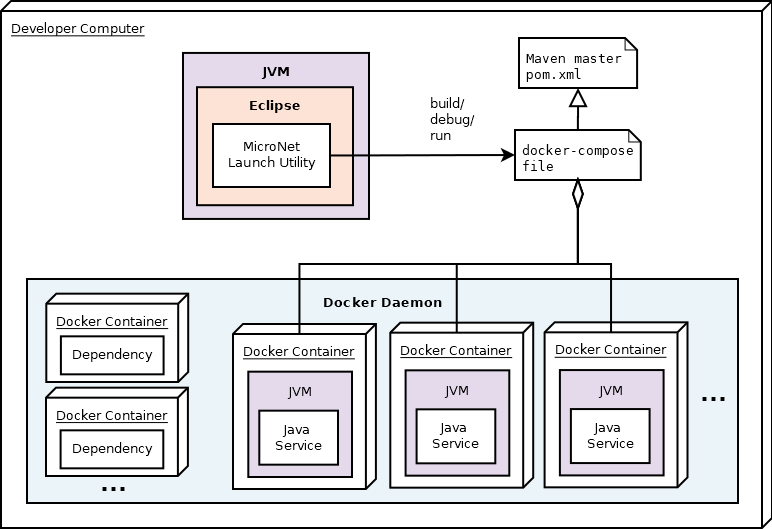
\includegraphics[width=\textwidth]{images/architecture/DeploymentLocalContainerized}
	\caption{Local containerized deployment of a MicroNet driven application.}
	\label{fig:deployment_local_containerized}
\end{figure}

\autoref{fig:deployment_local_containerized} shows how an application is
composed and deployed in the local containerized mode.

\paragraph{Cloud Containerized}

The final step of \ms{} application deployment is cloud deployment. The idea
behind application containerization is that this process is meant to be
deterministically reproducible on different systems. Therefore if the
application is working in the local containerized configuration the cloud
configuration can be achieved in a similar way.

MicroNet does not provide any out-of-the box solution to automatically deploy an
application in the cloud. This is because of the variety of
different infrastructures that can be used to deploy MicroNet. But the
deployment is prepared by MicroNet so it can be done with very few console
commands via SSH.

Due to the restrictions mentioned in \autoref{sub:zero_buget} the production
environment of \mn{} is a virtual Linux server in the HSR cloud. The cloud
deployment process is mainly based on this environment. Since this a very
general setup the process can easily be reproduced on other environments.

In order to deploy a MicroNet \ms{} application the developer must perform the
following steps under the assumption that the server runs a fresh Linux
installation.

\begin{itemize}
  \item Install: Docker Engine, Java, Maven and Git.
  \item Initialize docker swarm (master and worker machines).
  \item Pull the game application repository via Git (containing all service
  projects and the shared folder).
  \item Build the application class files using the master .pom file (annotation
  processing and code generation is performed during this step).
  \item Containerize the application using docker-compose \gls{api} and the generated
  docker-compose file.
  \item Launch the application in Docker Swarm using the docker stack \gls{api}.
\end{itemize}

\begin{figure}
	\hspace*{-0.8cm}
	\centering
	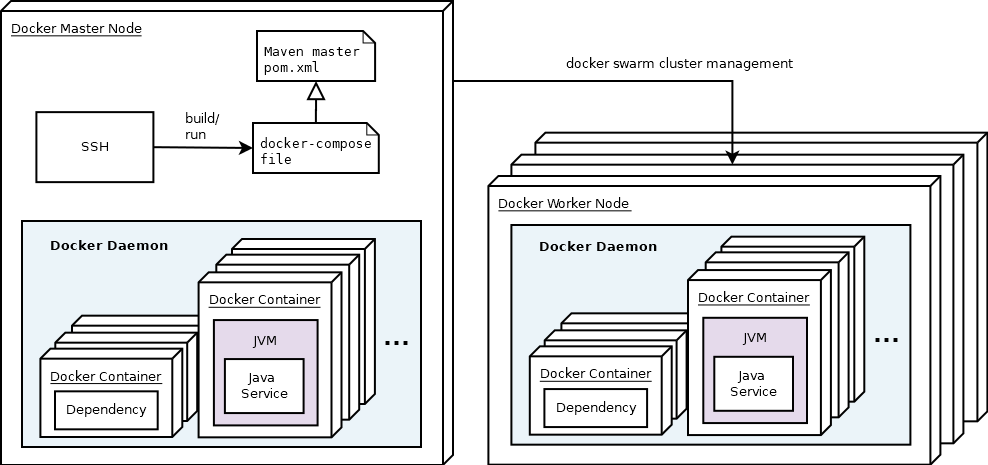
\includegraphics[width=1.1\textwidth]{images/architecture/DeploymentCloudContainerized}
	\caption{Cloud containerized deployment of a MicroNet driven application.}
	\label{fig:deployment_cloud_containerized}
\end{figure}

This sounds like a lot of steps but in fact the process is reasonably quick and
only requires very few console commands which can be looked up in the MicroNet
documentation \cite{micronet2017doku}.
\autoref{fig:deployment_cloud_containerized} gives an impression on how such a
docker-swarm environment may look like.

\subsubsection{Model Editor}

The \textit{Model Editor} is the last feature that was introduced in MicroNet
tools. It is the final solution for how to cope with logical \ms{} composition
through the \textit{Shared Model} in a visual way. Since the game model is
designed to be mainly machine-readable it is not suited to be directly edited in
the underlying \gls{json} files. The \textit{Model Editor} is designed to allow
convenient defining and editing of the model in a way which is especially useful
for \og{} application.

The \textit{Model Editor} is basically a graph editor visualizing a direct
representation of the game graph to allow extending and changing the graph. The
graph has three root nodes each of which span a model tree: the parameter code
list, the \textit{Template Tree}, and the \textit{Prefab Tree}.

\paragraph{Parameter Code List}

The parameter code tree is simply a flat list of String constants which define
all the parameter codes used throughout the application. This global approach
allows the substitution of the parameter codes strings with numbers, which is
more space efficient. Since parameters are used very often this has a noticeable
impact on the bandwidth requirements of an application.

\paragraph{Template Tree}

The \textit{Template Tree} allows to edit the game's \textit{Template Types}
using graph editing. Object Types defined using the \textit{Template Tree} can
be used for message transfer and persistence. \textit{Template Type} are
descriptions of domain objects and are used to generate \textit{Shared Model}
classes (POJOs) during code generation.

A \textit{Template Type} consists of a set of fields that may be of the
following types: STRING, NUMBER, BOOLEAN, CHAR, ENUM, LIST, SET, MAP, and
COMPONENT. The types are derived from the Java types since they are well
documented and can be redefined in other programming languages using the Java
language specifications.

The COMPONENT type can be any other \textit{Template Type}. A component is
represented as a field in the data class. Also \textit{Template Types} can be
derived from other \textit{Template Types}. The derivation is realized using
regular Java inheritance. \autoref{fig:model_view} shows the \textit{Model
Editor} which can be used to manually edit the \textit{Template Tree}.

\begin{figure}
	\centering
	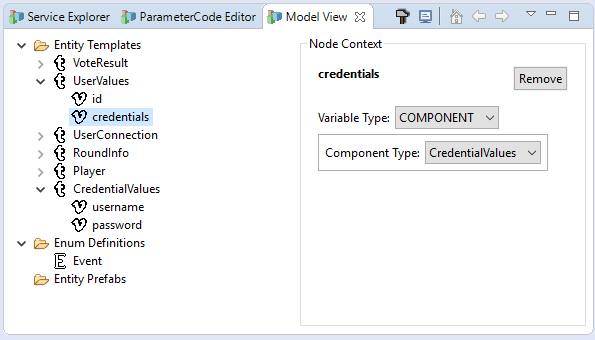
\includegraphics[width=\textwidth]{images/tools/ModelView}
	\caption{\textit{Template Type} editing with the MicroNet \textit{Model Editor}.}
	\label{fig:model_view}
\end{figure}

\paragraph{Prefab Tree}

The \textit{Prefab Tree} is a ``physical'' instantiation of the game graph. It
contains actual instances of \textit{Template Types}. This can be used by game
designers to pre-define game objects that are later used in the game. The
\textit{Prefab Tree} is directly compatible with the serialization component
provided by MicroNet. The generated model classes which represent the
\textit{Template Types} can be used to directly serialize and de-serialize game
objects which are part of the prefab-tree. The serialized data can directly be
stored in the database or be used as a payload or as parameters for message
transfers.

The \textit{Prefab Tree} can either be persisted in the file-system or persisted in the
database in \gls{json} format. The \textit{Prefab} approach allows for very
convenient and consistent handling of game data both during development and
operation.


\subsection{Example Game}

MicroNet provides a simple but complete example of an \og{}. Although the sample
game is very simple it gives a good overview over the functionality of MicroNet.

The sample game is a guessing game which is played in rounds of 15 seconds.
In each round the players have to guess a number between 1 and 100. The players
receive a score based on the proximity of the guess to the number. The score of
all player is shown in a scoreboard. 

The game client of the sample game is a standalone Java application using the
Laterna console gui library. Laterna allows to develop window based GUIs for the
terminal. This allows to run the game client also on server environments
through the command line. \todo{screenshot}

\autoref{fig:sample_game_flow} shows the communication of the sample game. The
numeric sequence is the communication flow of a player vote and the capital
letter sequence is the round control communication.\\

\begin{figure}
	\centering
	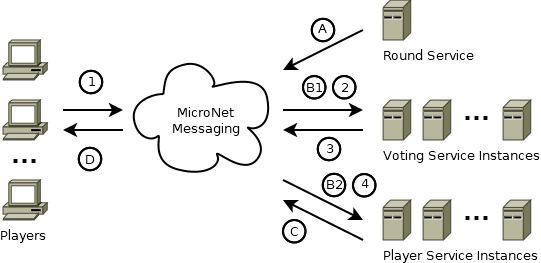
\includegraphics[width=\textwidth]{images/architecture/SampleGame}
	\caption{Communication flow of the Example Game.}
	\label{fig:sample_game_flow}
\end{figure}

The round control communication flow:

\begin{enumerate}[label=\Alph*.]
  \item The round service broadcasts a new new round event. The new round event
  contains the guessed number for the next round.
  \item \begin{enumerate}[label=\arabic*.]
    \item All voting services receive the new round event and store next the
    guess number in memory.
  	\item One player service receives the new round event to issue a score
  	broadcast. The scores of all players are available through the session store.
  \end{enumerate}
  \item The player service which received the new round event broadcasts a score
  update event to all participating players.
  \item Each player received the score update and updates its scoreboard
  accordingly.
   
\end{enumerate}

The player voting communication flow:

\begin{enumerate}
  \item The player sends his vote to the game application.
  \item The voting service instances compete for the vote messages.
  \item The processing voting service instance sends a score update message to
  an arbitrary player service.
  \item The processing player service persists the vote using the session store.
\end{enumerate}

It has to be mentioned that the round service is a singleton service. This is
necessary to ensure that the new round event is broadcast only once. Problems
like this are very common in distributed game development. To ensure the
stability of the application despite having singleton services can be quite a
challenge. One strategy is to keep singleton services as small as possible to
leave little room for failure. In the case of a failure the composition engine
must ensure that the singleton service is restarted. 

A singleton service must be designed in a way that no crucial data is lost upon
service failure and it must be possible to recover the state of a singleton
service after service failure.




\subsection{Testability}

The testing concept for \ms{} applications relies on the integrated in the
Maven build process of the application. Since the services expose their API as
Java functions testing can bypass networking for testing. The handler functions
are called directly in the test classes.

One problem with \ms{} testing is the access to the database. To spare the
developer with the need to mock the database a containerized database that can
be started before any tests are executed.
 


\newpage
\section{Validation of Survey}



\subsection{Results of Statistical Testing}

\subsection{Interpretation of Statistical Results}

\chapter{Conclusion}

In this concluding section of the thesis I want to give my own opinion about the
topics \mss{} and \ogs{}. My own view on the topics is heavily influenced by my
background as a programmer and hobby game developer.

\section{Summary of Findings}

The research motivation for this thesis is \ms{} development, especially
\ms{} composition and deployment. In these two areas I gathered a lot of
knowledge during this thesis and in this section I want to share the findings
that i find most relevant. These findings represent my attempt to answer the
knowledge questions in \autoref{sub:hypothesis}.

\subsection{Usability of a \ms{} for Online Games}

\noindent
\textbf{Can an Online Game run in a \ms{} environment?}

Yes, it is possible to run an \og{} in a \ms{} environment. I has already been
done in the industry (\cite{pronschinske2015turbine}) and MicroNet is an example
on how to accomplish this.\\

\noindent
\textbf{Is a Microservice influenced architecture suitable to design an Online
Game?}

The design of a \mss{} application heavily influences the way \ogs{} are
developed. This type of architecture forces the developer to split up the game
logic into small shard of \ms{} ``size''. This enforces that large domain chunks
which have high cohesion (like for example all player related functionality)
have to be split into smaller chunks. It is sometimes difficult to achieve
needed functionality this way. A good example of this aspect is the shop service
which served is explained in detail in \todo{autoref thesis 2}.

\noindent
\textbf{Is the added complexity during development tolerable?}

\ms{} indeed  adds an overhead during development. This effort pays off later
since scaling and extending of the application are simplified greatly. The added
effort occurs mainly at the beginning of a game project for example to set up
the continuous integration work-flow. For large teams (AAA companies) this
overhead can be neglected since a DevOps team can positioned to cope with these
boiler plate tasks beforehand and during the project.

For small teams (independent developers) however the overhead can be quite
troublesome. Once the development environment for \ms{}is set up the effort is
equivalent to regular \og{} development. MicroNet is aimed to fill exactly this
gab and make it easier to start with \ms{} driven \og{} development.

\noindent
\textbf{Do \mss{} have enough performance to drive a fast-paced \ogs{}?}

This question is very hard to answer in the context of this thesis. To give
sophisticated assumptions about the performance of a \ms{} application a  
full-fledged test game and a large enough group of testers is needed. The
Spacegame which I developed in my free time is not compete enough to fulfill
this role. During this semester i had basically no time at all to improve the
stability of the Spacegame to a level suited for TAR. Also the acquisition of
testers can be quite challenging since it involves a lot of community work
which is out of scope for this thesis.



\subsection{Reasons to use \mss{}}

\subsection{Tools are a Big Help}

\subsection{Achieving Platform Independence}

\section{Conclusions Drawn my Results}

\subsection{Hypotheses Verification}

\subsection{\ms{} Tenet Guidelines}

\subsection{Contradictions to a Pure \ms{} World}

\subsection{Questions for Practitioners}

\section{Recommendations for Further Research}

\bibliography{lit}
\bibliographystyle{alpha}

\printglossaries

\listoffigures

\appendix
\chapter{Project Plan}

\begin{figure}[H]
	\hspace*{-1.6cm}
  	\centering
  	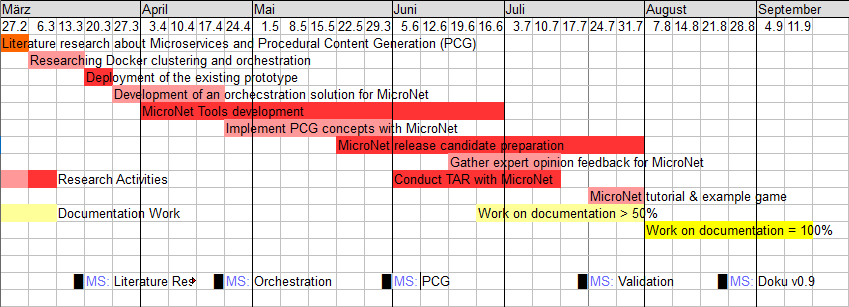
\includegraphics[width=1.2\textwidth]{images/ProjectPlan}
  	\caption{The project plan as defined at the beginning of this thesis.}
  	\label{fig:project_plan}
\end{figure}


\autoref{fig:project_plan} shows the project plan how it was established at the
beginning of this thesis. Unfortunately the project plan could not be fully met
and several activities were delayed.

Most noticeably \gls{pcg} was planned to be a prominent topic during this semester but
due to the workload introduced by composition and deployment topics the time
budget for \gls{pcg} shrank close to zero. This implies that the literature
about \gls{pcg} at the beginning of this thesis was a bit of a waste of time.

The work on the documentation also required a lot more effort than anticipated
because the documentation tended to grow quite rapidly. As a consequence all
other activities were suspended during July.

MicroNet Tools development was mostly on track but due to time consumption of
documentation work the final release of MicroNet and the associated
documentation were delayed until the end of August. Since the validation through
expert opinion relied on MicroNet being fully functional the validation survey
was executed much too late by the end of August when this thesis was almost
over.

All other activities were mainly on track and especially \gls{tar} was executed
just as planned in the middle of June.  

\chapter{Time Report}
\chapter{Personal Report}

\end{document} 